\documentclass[oneside,a4paper,12pt, colorinlistoftodos]{article} % Gibt an: Papierformat, Schriftgröße 
\usepackage{thesis}
\usepackage{breakcites}
\usepackage{pdfpages}
\usepackage{titlesec}
\usepackage{graphicx}
\usepackage{hyperref}
% Hier werden die Abkürzungen definiert. Sofern ein Abkürzungsverzeichnis verwendet wird bitte entkommentieren.
\newacronym{aifb}{AIFB}{Institut für Angewandte Informatik und Formale Beschreibungsverfahren}
\newacronym{kit}{KIT}{Karslruher Institute für Technologie}
\newacronym{cii}{CII}{critical information infrastructure}
\newacronym{dlt}{DLT}{distributed ledger technology}
\newacronym{ts}{TS}{typescript}
\newacronym{ssr}{SSR}{Server Side Rendering}
\newacronym{ssg}{SSG}{Server Side Generation}
\newacronym{isr}{ISR}{Incremental Static Regeneration}
\newacronym{seo}{SEO}{Search Engine Optimization}
\newacronym{rfc}{RFC}{Request for Comments}
\newacronym{dx}{DX}{Developer Experience}
\newacronym{gui}{GUI}{Graphical User Interface}
\newacronym{cli}{CLI}{Command Line Interface}
\newacronym{abi}{ABI}{Application Binary Interface}


\begin{document}
% \setlanguageGerman % Sprache einstellen.
\setlanguageEnglish

% Hier kommt der ganze Vorspann. Bei Verwendung von Abkürzungs-, Abbildungs- oder Tabellenverzeichnisse bitte in dieser Datei entsprechend entkommentieren.
\pagenumbering{roman}
\begin{titlepage}
% font / Schriftart
%------------------	


\begin{figure}[htbp]
  %\centering
  \begin{minipage}[b]{7cm}
    \ifthenelse{\boolean{english}}{
\includegraphics[height=1.8cm]{images/kit_logo_en}}{
\includegraphics[height=1.8cm]{images/kit_logo_de}}
  \end{minipage}
  \begin{minipage}[b]{8.5cm}
	\begin{flushright}


    
\includegraphics[height=1.8cm]{images/aifb_logo}  
		\end{flushright}
  \end{minipage}
\end{figure}

\vspace*{2.5cm}
\begin{center}
		{\textbf{\Huge \ifthenelse{\boolean{english}}{SPECK-Hackathon}{SPECK-Hackathon}}}
		\vspace*{1cm}\\
		{\Large \ifthenelse{\boolean{english}}{Hackathon Documentation}{Hackathon Dokumentation}}\\[1cm]
		{\Large \ifthenelse{\boolean{english}}{by}{von}}\\[1cm]
		%\vspace*{1cm}
		{\huge Philip Heller, Hichem Ben Aoun}\\[0.5cm]
		{\Large \ifthenelse{\boolean{english}}{Degree Course: Information Systems M.Sc.}{Studiengang: Wirtschaftsingenieurwesen}}\\[0.25cm]
		%TODO MatNr angeben
		{\Large \ifthenelse{\boolean{english}}{Matriculation Number}{Matrikelnummer}: 2111444, 2480704}\\
		\vspace*{1cm}
		{\Large\ifthenelse{\boolean{english}}{
			Institute of Applied Informatics and Formal Description Methods (AIFB)
			\\[0.5cm]
			KIT Department of Economics and Management\\[0.3cm]
            Words: 7500}{
			Institut für Angewandte Informatik und Formale Beschreibungsverfahren (AIFB)
			\\[0.5cm]
			KIT-Fakultät für Wirtschaftswissenschaften\\[0.3cm]
            Words: 7000
            }
		}
	\end{center}
	\vspace*{1cm}
\Large{
\begin{center}
\begin{tabular}[ht]{l c l}
	
  %TODO Referent/-in angebenn
  %Referent/-in sind die Professoren, die die Arbeit bewerten.
  \ifthenelse{\boolean{english}}{Advisor}{Prüfer}: & \hfill  & 
M. Sc. Niclas Kannengießer \\
  %Referent/-in sind die Professoren, die die Arbeit bewerten.
  \ifthenelse{\boolean{english}}{Second Advisor}{Zweiter Prüfer}: & \hfill  & 
 \\
  %TODO Betreuer/-in angeben
  %TODO Abgabedatum angeben
  \ifthenelse{\boolean{english}}{Submitted}{Eingereicht am}: & \hfill  & \today\\
 
\end{tabular}
\end{center}

}


%\include{titel}
  \vfill
	
	\small{ KIT -- \ifthenelse{\boolean{english}}{The Research University in the Helmholtz Association}{Die Forschungsuniversität in der Helmholtz-Gemeinschaft}
} \hfill
	\small{\textbf{\url{www.kit.edu}} }
\end{titlepage}
%Für den Fall eines Vorworts entkommentieren:
%\mbox{}\thispagestyle{empty}

\vspace*{1cm}

{\Large \textbf{\ifthenelse{\boolean{english}}{Prologue}{Vorwort}}} 

\bigskip

\ifthenelse{\boolean{english}}
{\selectlanguage{english}
In English theses, German prologue is probably to be used, so paste it here. \blindtext
}
{\selectlanguage{ngerman}
Hier könnte ein Vorwort stehen.
}
% \thispagestyle{empty}\section*{\ifthenelse{\boolean{english}}{Abstract}{Zusammenfassung}}
An dieser Stelle erfolgt eine knappe Zusammenfassung der vorliegenden Arbeit ([engl.] Abstract), die maximal ca. 200 Worte umfassen sollte. Der Sinn und Zweck dieser Zusammenfassung liegt darin, einem interessierten Leser die Entscheidung zu erleichtern, die vorliegende Arbeit überhaupt zu lesen bzw. vor dem Lesen der Arbeit erst einmal in Erfahrung zu bringen, worum es dabei geht. Also eine knappe, motivierende Hinführung zum Problem und wie Sie es gelöst haben.

Wenn Sie eine Zusammenfassung schreiben, bedenken Sie, dass diese oft auch alleine publiziert wird, d.h. sie sollte unabhängig vom nachfolgenden explizit dargestellten Inhalt der Arbeit für den Leser verständlich sein. Daher ist es immer sinnvoll, diese Zusammenfassung erst ganz am Ende zu schreiben, wenn Sie die eigentliche Arbeit bereits abgeschlossen haben. todo include in real paper
%\setcounter{page}{3}
\tableofcontents\newcounter{roemisch} %\setcounter{roemisch}{\value{page}}
% Für den Fall von Abkürzungs-, Abbildungs- oder Tabellenverzeichnissen entkommentieren
\ifthenelse{\boolean{english}}
{\cleardoublepage\printnoidxglossary[type=acronym,sort=letter,nonumberlist,title={List of Abbreviations}]}
{\cleardoublepage\printnoidxglossary[type=acronym,sort=letter,nonumberlist,title={Abkürzungsverzeichnis}]}
%\cleardoublepage\listoffigures
%\cleardoublepage\listoftables
%\cleardoublepage\setcounter{page}{2} 
\cleardoublepage
\pagenumbering{arabic}

% Füge hier die Kapitel per Verweis ein. Der Befehl \include fügt die angegebene tex-Datei an der jeweiligen Stelle ein. Die eingefügte Datei wird als normaler Teil des Quelltextes mitverarbeitet und ist daher LaTeX-Code (ohne Vorspann und \begin{document}...\end{document}).

\clearpage

\section{Introduction}


SPECK is an innovative blockchain-based supply chain solution, purpose-built to revolutionize the way meat, specifically pig products, are managed throughout their lifecycle. Combining state-of-the-art technology with the core demands of the meat industry, SPECK provides unprecedented transparency, traceability, and efficiency to all stakeholders in the pig production supply chain.

Leveraging the power of the Ethereum network, SPECK utilizes ERC-721, a free and open standard that describes how to build non-fungible or unique tokens on the Ethereum blockchain. Each unique token represents an individual pig or a specific pork product. This ensures an unmatched level of accountability, as each token can be traced from its origin through the entire supply chain.

The innovative use of ERC-721 allows for the individual identification of each pig or pork product, meaning that every single piece of meat can be tracked from farm to fork. The unique token attached to each product contains vital information such as the animal's birthplace, diet, health records, and processing and transportation details. This offers consumers and stakeholders complete visibility and assurance about the quality, safety, and origin of their food products.

SPECK's functionality is not limited to the blockchain backend. It also features a robust and user-friendly front end, designed to make the system accessible to everyone from farmers and processors to retailers and consumers. This interactive interface allows users to effortlessly manage, track, and save pig products at every stage of the supply chain.

The next section delineates the requirements, further subdivided into functional and non-functional aspects. The third section outlines the assumptions made during the project conception, detailing the trust model, Threat model, Project-specific assumptions, and Conceptualization. The Implementation forms the core of the document, exploring the technical elements of the project. It dives into specifics about the techstack, which includes the front-end and smart contract framework, the project Architecture, the process of dockerization, and an overview of the Contracts involved, with a deeper focus on the two smart contracts \textit{OrganizationAuthenticator.sol} and \textit{Speck.sol}. This section also examines the Front-end, dev-pages, and public pages of the project. Future work, including aspects like view restriction, Gas optimization, Decentralized data storage, Change in Organization Data, Transfer proposal, and additional front-end features, is discussed towards the end.

\section{Requirements}
\subsection{Functional Requirements}

% \begin{itemize}
%     \item Consumers and organizations must be able to trace which animals were used in the making of specific food products.
%     \item Consumers must be able to trace which organizations participated in the production of specific food products.
%     \item Consumers must be able to view animal-welfare data of the organizations the animals have been to.
%     \item Consumers and organizations must be able to view emissions of companies that participated in the production of food products.
%     \item Consumers and organizations need to be able to view animal-related data (e.g., genetics of the animal, medication). The data is added gradually from the companies along the supply chain).
%     \item Consumers and organizations need to be able to access animal-related data and product-related data through a graphical user interface.
%     \item All companies must be able to upload animal-related and organization-related data to the SPECK system.
%     \item Organizations must be able to add attributes to animals and food products in the SPECK system.
%     \item Organizations must not be able to physically delete animal attributes and product attributes in the SPECK system.
%     \item Organization-related data (i.e., animal-welfare indices and emissions) must be updated once a year.
%     \item Organizations are able to trace individual animals and food products.
%     \item Organizations must be authenticated by a trusted third party (i.e., an authenticator).
% \end{itemize}

In the SPECK system, both consumers and organizations are provided with the ability to trace the origin of specific food products, down to the individual animals used in their production. Further, consumers are empowered with the ability to track which organizations participated in the making of specific food products, lending to increased transparency in the supply chain.

This system also caters to the growing demand for information regarding animal welfare, enabling consumers to view the animal-welfare data of the organizations the animals have been through. Similarly, both consumers and organizations can access data about the emissions produced by companies involved in the food products' production, promoting environmentally conscious choices.

Animal-related data, such as the animal's genetics and medication history, are added progressively by companies along the supply chain. This data, along with product-related information, is easily accessible through a graphical user interface, facilitating comprehension and decision-making for both consumers and organizations.

Companies are required to upload animal-related and organization-related data to the SPECK system, enhancing the depth and breadth of information available. Organizations are permitted to add attributes to animals and food products within the SPECK system, fostering a detailed representation of the products. However, it is important to note that they cannot physically delete these attributes, ensuring the integrity of data.

Organization-related data, such as animal-welfare indices and emissions, are updated annually, ensuring the information's relevancy. Additionally, organizations have the capability to trace individual animals and food products, which aids in managing supply chains more effectively.

A crucial aspect of the SPECK system is the requirement for organizations to be authenticated by a trusted third party, known as an authenticator. This process adds another layer of credibility to the information presented within the system.


\subsection{Non-functional Requirements}

% \textbf{Availability}
% \begin{itemize}
%     \item All data managed via the SPECK system must be highly available.
% \end{itemize}  

% \textbf{Integrity}
% \begin{itemize}
%     \item  Transaction data about animals must not be mutable.
%     \item Modification of animal or organization-related data must be recognizable by recipients.
%     \item Transactions stored in the ledger must not be mutable.
% \end{itemize}

For the SPECK system, Availability and Integrity are paramount. In terms of Availability, it is a requirement that all data managed through the SPECK system is highly available. This ensures that necessary information is accessible when needed, thereby facilitating efficient operations and decision-making processes.

Integrity, on the other hand, covers a few critical aspects. Firstly, transaction data about animals must remain immutable. This safeguards the accuracy of the data and prevents unauthorized alterations. Secondly, any modifications made to animal or organization-related data must be readily identifiable by recipients. This promotes transparency and allows users to be fully aware of any changes made. Lastly, transactions stored in the ledger must also be immutable. This principle maintains the veracity of the ledger and ensures that its records remain reliable and uncompromised.

\section{Assumptions}
\subsection{Trust model}
% As described in the speck doc:

\begin{itemize}
    \item Companies are incentivized to share data via the SPECK system.
    \item Companies have their own information systems in which they store all data that should be treated as confidential, including billing data and detailed customer data. We assume such information systems as secure.
    \item Companies independently take care of the key management of private keys or mnemonics for their wallet
    \item The consortium of companies in the SPECK system agreed on a set of trusted authenticators which are deposited in the organization list.
    \item All RFIDs used to identify animals are unique.
    \item Companies can contact each other via communication channels external to the SPECK system.
    \item Companies only store correct data(e.g., animal welfare score).
    \item Companies do not create shadow trees from already exhausted product states (i.e. vertices in product tree) 


    
\end{itemize}

\subsection{Threat model}
% As described in speck doc

\begin{itemize}
    \item Nodes may be arbitrarily unavailable (e.g., due to crashes).
    \item Companies manipulate data stored in the distributed ledger (e.g., to obfuscate bad animal welfare scores).
    \item Companies steal the identity of other companies in order to publish fictitious production data, thereby damaging the reputation of the organization concerned in the public eye.
    \item Companies modify entries in their local database that stores the ledger (e.g., to obfuscate bad animal welfare scores).
    \item Companies transfer the same product to multiple companies subsequent in the supply chain(e.g., to fake transfers).
    \item Shadow trees may be created
    
    
\end{itemize}

\begin{figure}[bth]
    \centering
    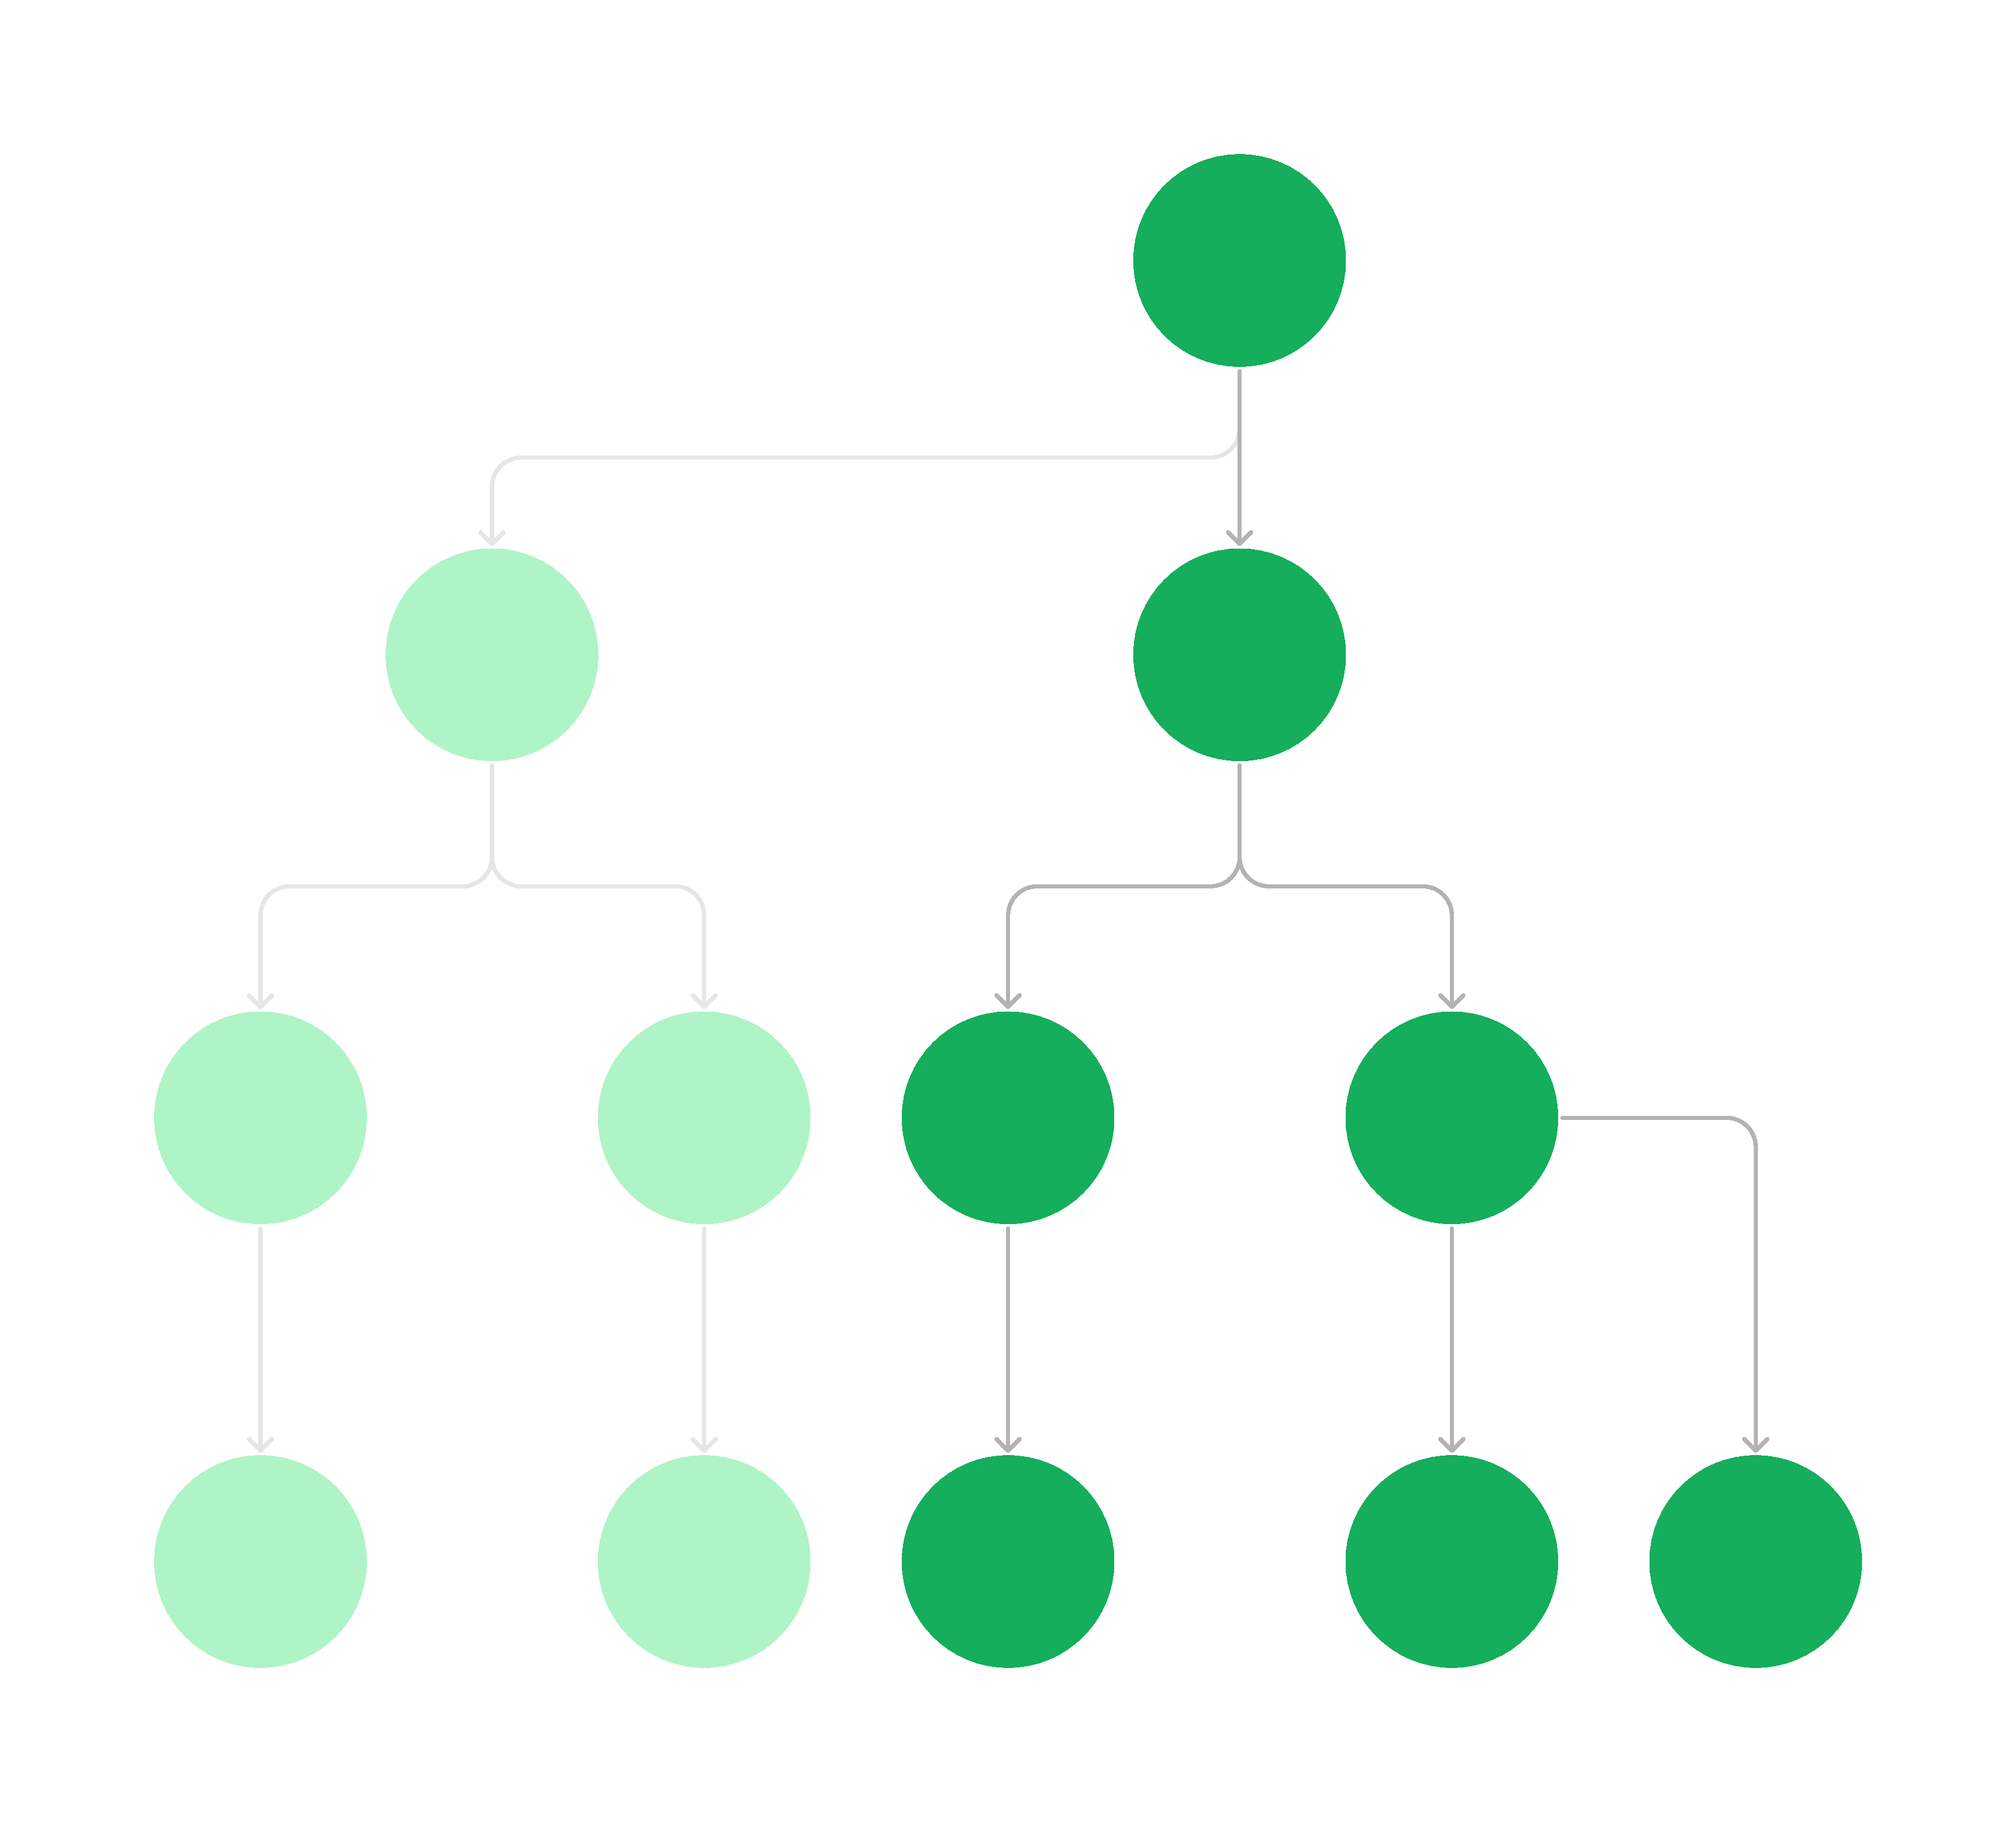
\includegraphics[width=0.5\textwidth]{images/shadow_tree.pdf}
    \caption{Example of a shadow tree}
    \label{fig:shadow_tree}
\end{figure}

\subsection{Project specific assumptions}\label{se:project_assumptions}

The SPECK project was initiated with a few assumptions central to its design and functioning. At the core of our endeavor is the desire to trace and present the entire lifecycle of a pig, from birth to the final product.

However, to make the system more accessible and less complex, we've simplified certain aspects. For instance, we've streamlined the process of transferring a pig from one entity to another (peers), so it's more user-friendly and doesn't become a bottleneck in the system's operation.

Despite our comprehensive approach, we consciously decided to exclude a few elements from the proof of concept (PoC) stage. It's important to note that this exclusion doesn't reflect oversight but a deliberate decision based on various factors such as feasibility, priority, and project timeline. These elements may be revisited and incorporated in future versions (see \ref{se:future_work}).

Another key assumption made during the conception of the SPECK project is the level of technical competence of the users, both organizations and individual consumers. The system assumes that users have the necessary technological knowledge to interact with the platform, input data where necessary, and interpret the information provided.

The operation of SPECK also relies on the assumption of stable and robust internet connectivity, as it's a blockchain-based system requiring constant data transfer. Additionally, it's assumed that all participating entities comply with relevant local and international regulations regarding animal welfare, food safety, and data privacy.

Furthermore, SPECK assumes that all participating organizations are comfortable with blockchain technology and recognize its value in ensuring traceability and transparency in the supply chain. And finally, we assume that consumers and organizations hold a deep concern for sustainability and animal welfare, influencing their purchasing or operational decisions based on the data provided by SPECK.

\subsection{Conceptualization}\label{se:conceptualization} 

During the conceptualization of the project, the team identified four key modules that form the foundation of the system.

The first module is the baseline, which involves managing the pig meat supply chain. This module is implemented in the \textit{Speck.sol} contract, which serves as the core component responsible for creating and tracking unique product tokens, representing individual pigs or specific pork products. It ensures transparency, traceability, and efficient management throughout the lifecycle of the products.

The second module is the organization validation, implemented in the \textit{OrganizationAuthenticator.sol} contract, as mentioned earlier. This module focuses on authenticating and registering organizations participating in the supply chain. It verifies the identity and authorization of organizations to ensure that only validated entities can interact with the system.

The third module is cumulative aggregation, which involves clustering products or animals into groups or clusters. This allows for the registration of products or pigs in bulks, streamlining the process and improving efficiency in managing large quantities of data within the supply chain.

Lastly, the fourth module addresses the confidentiality of certain attributes or product properties. It recognizes the need to protect sensitive information, such as medication details, animal welfare scores, or environmental data. This module ensures that access to specific attributes or properties is restricted only to authorized entities, maintaining confidentiality while providing transparency across the supply chain.

By conceptualizing the project into these modules, the team establishes a comprehensive framework that addresses various aspects of the pig meat supply chain, including authentication, traceability, efficiency, and data confidentiality.

\section{Implementation}

This section will describe the process for the creation of a PoC for the SPECK project and discuss choices for the techstack, the architecture and the different containerized components during the implementation of the project.

% \begin{enumerate}
%     \item Starting point (repo for drizzle w react)
%     \item Issues with that repo and why we decided to change things about it (making it necessary to opt for other libraries)
%     \begin{itemize}
%         \item CRA is kind of old, Meta-frameworks such as Nextjs have more out of the box while being kept simpler
%         \item The project was not correctly dockerized:
%         \begin{itemize}
%             \item not encapsulating the different responsibilities of components
%             \item installation at runtime instead of build time (slow cold starts and slow hot starts)
%             \item packages used are mostly stale (no changes in drizzle for years, missing a good documentation, no support for \gls{ts})
%             \item wanted to integrate a few qol libraries to simplify development (tailwindcss)
%         \end{itemize}
%     \end{itemize}
%     \item decided to create a generic PoC that can handle a simple storing of a string (SimpleStringStore)
% \end{enumerate}

At the beginning of the hackathon, a demonstrative repository using the Truffle suite (Ganache, Truffle and Drizzle) was provided as entry point and proof of concept to get started \cite{drizzleWithEvents}. However, during the early stages of conceptualizing and exploring options (creation of a SPECK-PoC) a few problems and limitations of the exemplary repository were identified:

\begin{enumerate}
    \item \cite{drizzleWithEvents} uses create-react-app \cite{createReactApp} (slower as it still uses webpack instead of modern solutions such as vite or turbopack, fewer features for quality of life and \gls{dx})
    \item \cite{drizzleWithEvents} uses drizzle which has not been changed in 3-4 years, poorly documented, missing support for \gls{ts}
    \item \cite{drizzleWithEvents} does not work out of the box and has configuration overhead (has .env file that is not needed but needs to be configured)
    \item \cite{drizzleWithEvents} does not encapsulate the individual components into own containers (Ganache and Truffle are run in same container which is not best practice resulting in more complexity to manage containers, slower build times)
    \item \cite{drizzleWithEvents} installs dependencies during runtime instead of during build time (slow cold and hot starts)
\end{enumerate}

Therefore, the project dependencies and virtualization through Docker (ultimately also the architecture) were reworked to find fitting solutions addressing the problems described above. The individual issues live in different conceptual layers described in the following sections (see \ref{se:techstack}, \ref{se:architecture} and \ref{se:dockerization}). An early version of an exemplary application using the updated environment is tagged in \cite{wagmiExample}\footnote{Note, that a few things were changed in the final implementation of SPECK (see tag message).}. The final submission of the SPECK project is located in the repository in the main branch \cite{HellerAoun}.


\subsection{Techstack}\label{se:techstack}
In the exploration phase for a DLT, more specifically a Solidity project, different technologies have been looked at to find a suitable solution. These can be separated into the frontend and the blockchain. 

\subsubsection{Frontend}
For the frontend, Nextjs \cite{nextjs} was chosen. It supports \gls{ts} out of the box and leverages technologies used in large scale applications for \gls{seo} such as \gls{ssg}, \gls{ssr} and \gls{isr}. It also features a built in router, automatic code splitting and a rich ecosystem of plugins and popular tools. Though many of these tools are not strictly necessary for SPECK, these attributes made Nextjs a popular framework with a large community, a stable environment and integration of newest innovations in React. A great example is the use of component level client and server rendering that was introduced in React 18. Nextjs is the first large meta framework that implemented it as beta in a \gls{rfc}.\\
To simplify the styling process, Tailwindcss \cite{tailwind} was used. Tailwindcss is a utility class system that shortens the amount of css and helps creating consistent styling throughout the application. \\
For the interaction with web3-components, an alternative for drizzle was chosen. Unfortunately, drizzle does not support \gls{ts} and is poorly documented. It has also not seen any development activity lately. As alternative, Wagmi \cite{wagmi} was chosen. It supports \gls{ts} and delivers a large set of hooks that provide several updates in state kept track of by Wagmi. It reduces the complexity of interaction with smart contracts and the blockchain significantly resulting in greater \gls{dx}.

\subsubsection{Smart Contract Framework}
There are currently two large and popular frameworks commonly used and referenced for the development of web3 applications: Hardhat  and Truffle. Both frameworks deliver tools and interfaces for the development of smart contracts and complex applications. One advantage of hardhat is it's modularity and it's out of the box support for \gls{ts}. Truffle on the other hand comes with it's own suite of tools such as Ganache \cite{ganache} that are tightly coupled. \\
Due to a high degree of feature parity and in the name maintainability the Truffle suite was chosen for smart contract development. Thereby, the example project \cite{drizzleWithEvents} resembles the structure a bit more reducing complexity for developers who already work at the \gls{cii}. 


Choosing other dependencies solved the issues 1-2. Issues 3-5 are concerned with the dockerization and devops which are discussed in the following sections \ref{se:architecture} and \ref{se:dockerization}.
\subsection{Architecture}\label{se:architecture}
% \todo[inline, color=green]{@phil: Explain architecture of the project (how the different components play together, may be suitable to join with dockerization)}

The technologies listed above result in a cohesive mono repository. Figure \ref{fig:architecture_and_components} depicts the individual components and it's dependencies. Ganache serves as the local blockchain emulator, providing a simulated Ethereum network for testing and development purposes. It creates a sandbox environment where developers can create and manage test accounts, deploy smart contracts, and execute transactions. It comes as a \gls{gui} for users or as a \gls{cli}. This is more relevant for the dockerization in which Ganache is used through the \gls{cli} while developers can also opt to use a version on their host machine.
Truffle t simplifies the creation, compilation, testing, and deployment of smart contracts on the Ethereum network. Truffle's integration with Ganache enables developers to deploy and interact with their smart contracts in the local blockchain environment without manually passing the \glspl{abi} and binaries. It also provides the \glspl{abi} for the frontend.
Last but not least, Nextjs with Wagmi is used to create an extensive and accessible web application. The \gls{gui} is accessible through a number of browsers. Wagmi uses the \glspl{abi} and creates easy to use, typesafe hooks for the interaction with the smart contracts on the blockchain.



\begin{figure}[bht]
    \centering
    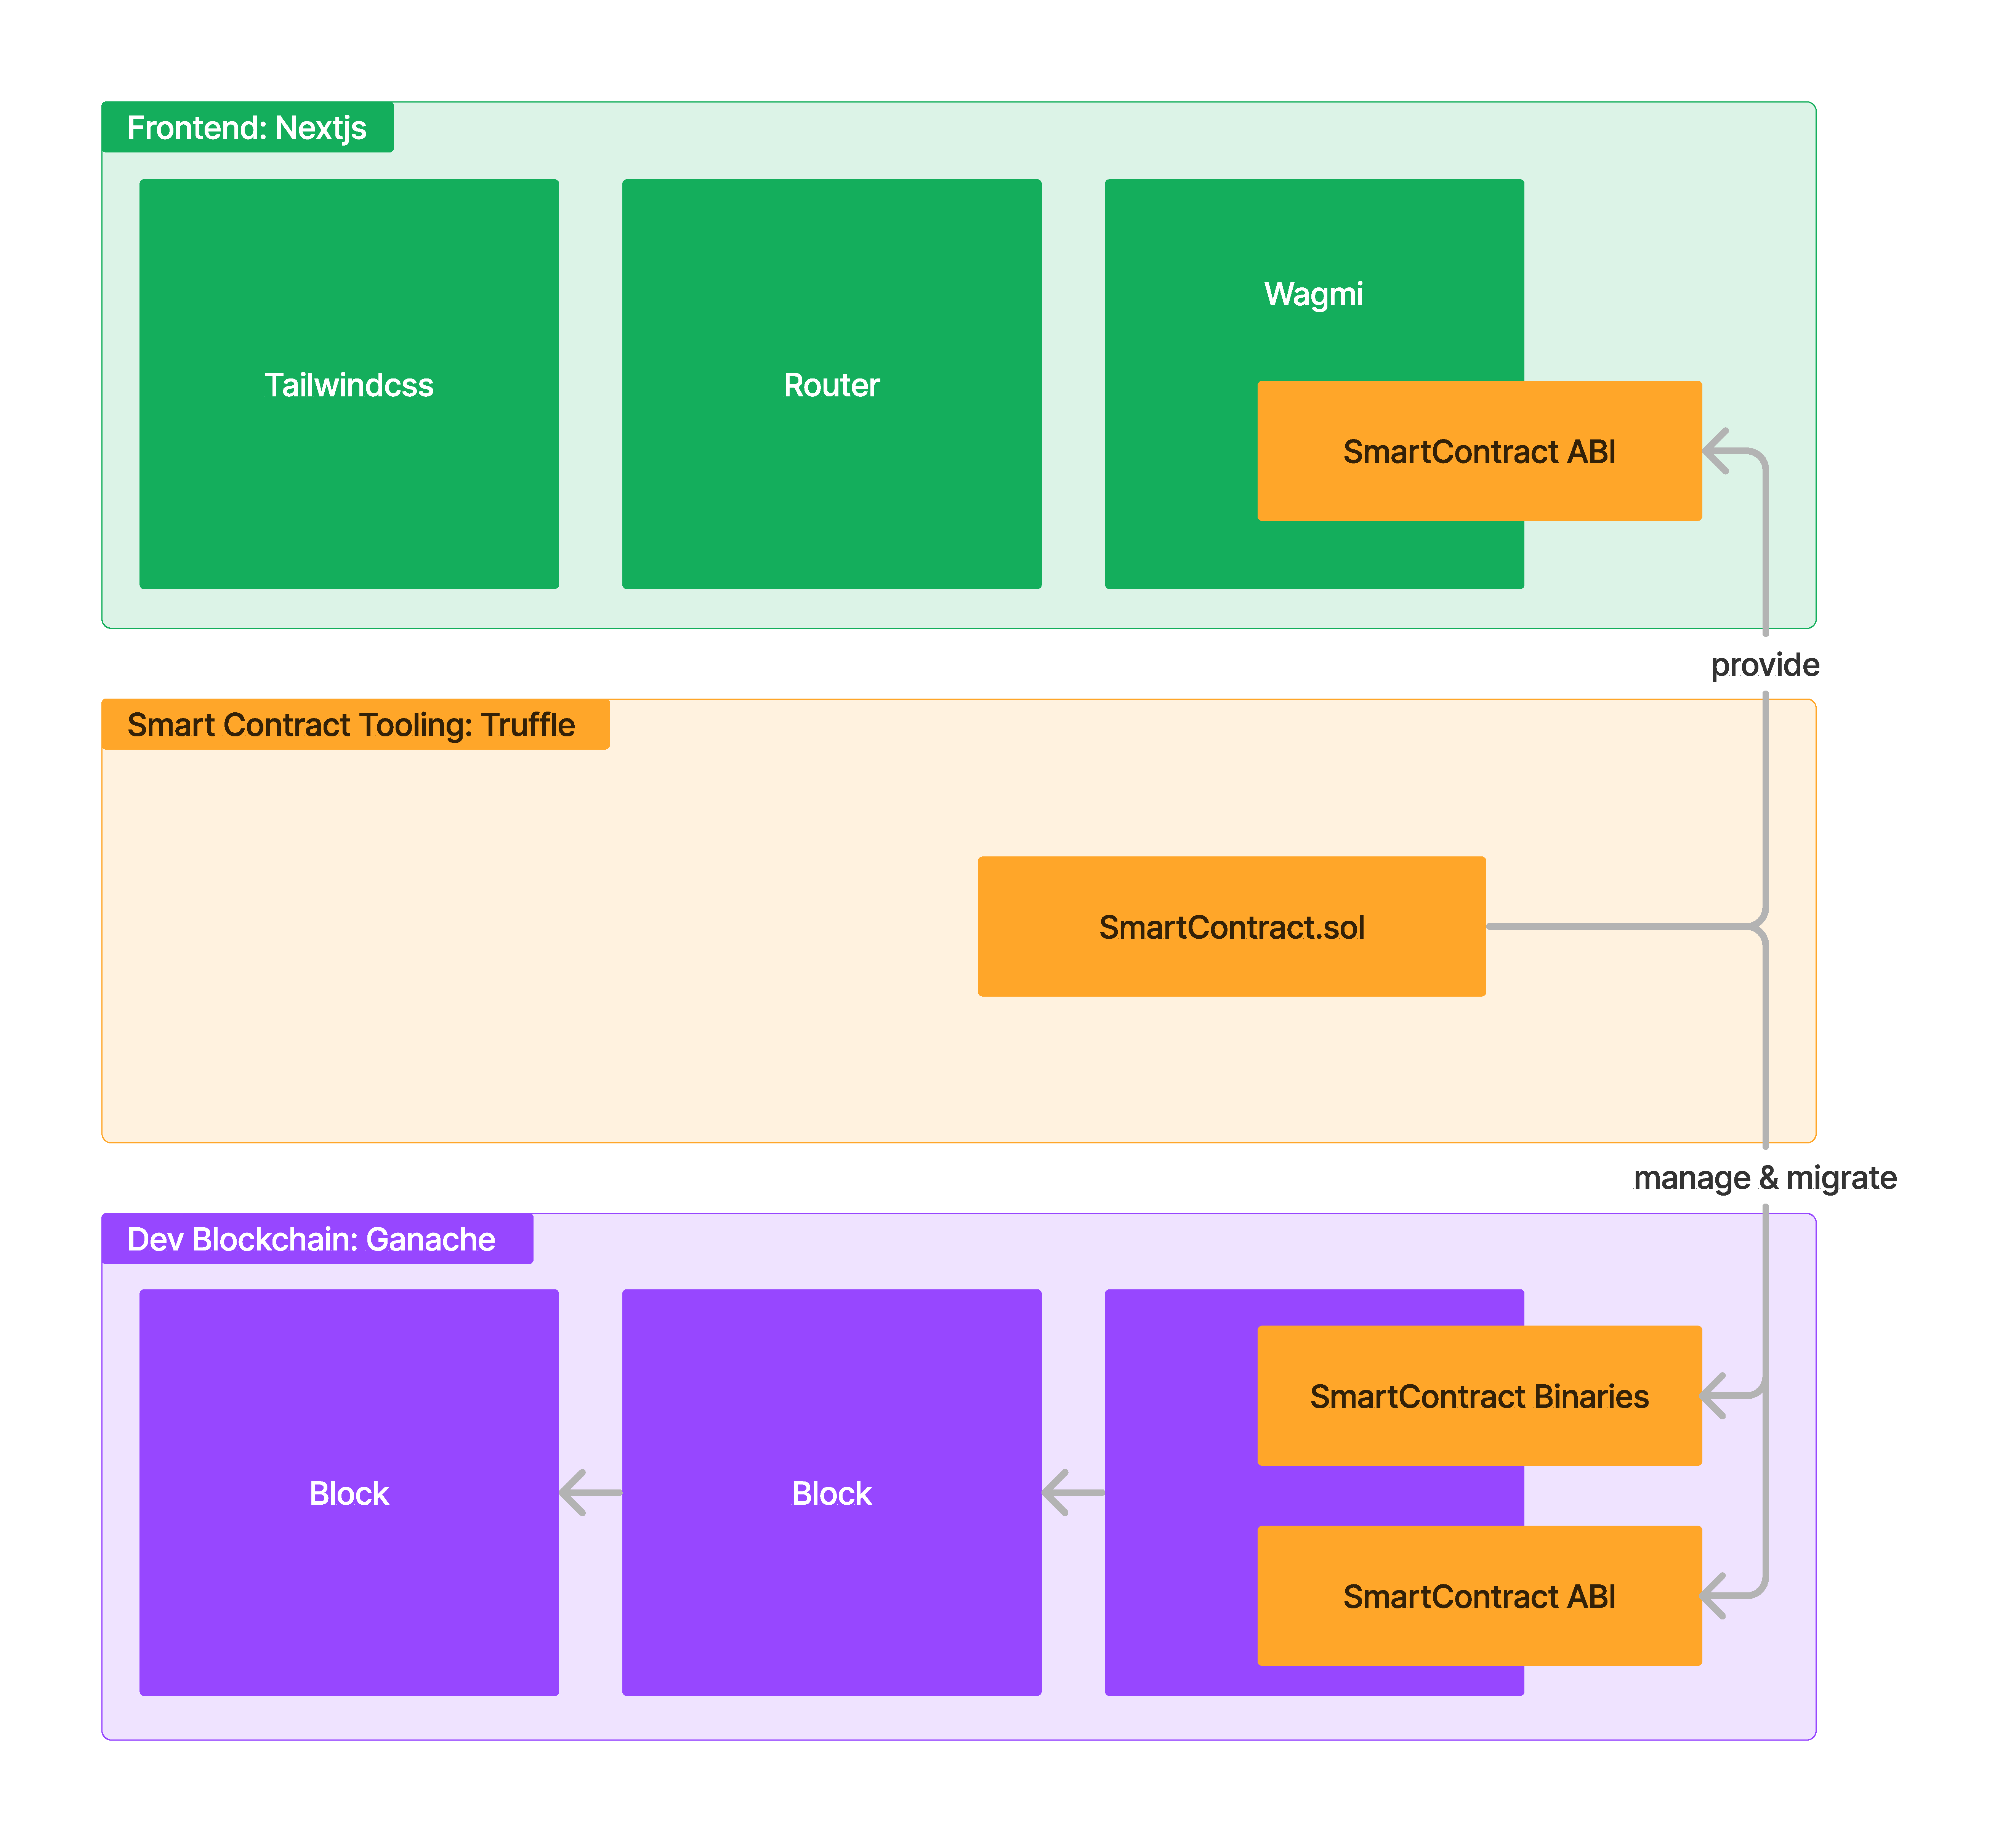
\includegraphics[width=\linewidth]{images/component_structure.pdf}
    \caption{Architecture of SPECK}
    \label{fig:architecture_and_components}
\end{figure}

\subsection{Dockerization}\label{se:dockerization}

Dockerizing the entire project helps the project in a couple of ways:
\begin{enumerate}
    \item \textbf{Easy reproducibility and consistentcy}\\
    Docker permits to easily create containerized environments and encapsulates all the necessary dependencies and configuations required in the project. Builds will be reproducible across different environments which eliminates "works on this machine" issues.
    \item \textbf{Simplified setup and configuration}\\
    Setting up the entire project environment with different frameworks and tools is often time consuming and error-prone. The dockerized project will eliminate manual installations and configurations and get developers started quickly (reducing onboarding time) through a standardized setup process.
    \item \textbf{Dependency management}
    Using different dependencies of a piece of software on the same host machine can be challenging. Docker simplifies the versioning and prevents issues with dependency conflicts of same dependencies. Each container has it's own environment that is independent.
    \item \textbf{Orchestration and spinning up the project}\\
    Spinning up a development environment with multiple interacting components is time consuming. Here, tools such as Docker Compose help by allowing to spin up the entire environment in a single command (docker-compose up). 
\end{enumerate}

 Most of the configuration is handled through the docker-compose.yml file in the repository \cite{HellerAoun}. It specifies the services, configurations, networking and volumes for persistent data. With this setup, developers can easily start the development with either a clean blockchain or with data persisted from last development session.

\subsection{Contracts}

The smart contracts used in this project are written in the programming language \textit{Solidity}. The functionalities are separated into two contracts based on the separation of concerns paradigm. The \textit{OrganizationAuthenticator.sol} contract handles the registration of organizations and their permission participate in the \textit{SPECK} system. This architecture allows other contracts or services to use the information stored on the \textit{OrganizationAuthenticator.sol} contract  to allow or restrict access to certain functionalities or information. The \textit{Speck.sol} is used for the saving and retrieving of product data and its history. Permission for the creation of products is derived from the registration data of the \textit{OrganizationAuthenticator.sol}.

\subsubsection{OrganizationAuthenticator}

The \textit{OrganizationAuthenticator.sol} contract is used to authenticate and register organizations. It allows organizations to request registration, and the contract owner can approve the registration requests. The contract also provides functions to retrieve organization data, check registration status, and manage organization requests.

The \textit{OrganizationAuthenticator.sol} smart contract serves a crucial role in the SPECK system as the gateway for organizations to participate in the network. This contract is employed to authenticate and register organizations, ensuring that only authorized entities have access and can contribute to the system after requesting registration (see figure 
 \ref{fig:registration_process}).



Key elements of this contract include:

\begin{enumerate}
    \item \textbf{Data Structs} \\
    The contract uses the data structure \texttt{Organization} struct to encapsulate and manage key information about an organization, including its name, type, email, address, and scores pertaining to animal welfare and environmental impact, among other details.
    \item \textbf{Organization Registration} \\
    A crucial function of this contract is to enable organizations to request registration. Upon request, the contract generates a unique ID for the new organization, stores their data, and marks the registration request as active. It then emits an event notifying that registration has been requested.
    \item \textbf{Organization Authentication} \\ 
    The contract contains methods to authenticate organizations based on their ID or Ethereum address. This function is important in maintaining the security and integrity of the \textit{SPECK} ecosystem.
    \item \textbf{Registration Approval} \\
    The contract also allows the contract owner to register an organization, given that the organization has an active registration request. Once registered, the organization's registration request is deactivated, and it is officially marked as registered.
    \item \textbf{Data Retrieval} \\
    Functions are provided to retrieve data about an organization, either based on its Ethereum address or the sender's address. Additionally, a list of all organizations that have requested registration can also be retrieved.
    \item \textbf{Total Request and Registration} \\
    The contract keeps track of the total number of organizations that have requested registration and those that have been registered.
    
\end{enumerate}

All of these functionalities contribute to the contract's primary goal of maintaining a trusted network of authenticated organizations that participate in the SPECK system, reinforcing the system's core values of transparency and accountability.

A detailed documentation of \textit{OrganizationAuthenticator.sol} is included in the appendix \ref{se:organization_authenticator.sol} or in the GitLab repository (\cite{HellerAoun}).


\subsubsection{Speck}
The \textit{Speck.sol} is a smart contract written in Solidity that represents a product as an ERC721 token, an Ethereum standard for non-fungible tokens. It allows authenticated organizations, as verified by the contract \textit{OrganizationAuthenticator.sol}, to create and transfer these tokens, which also contain detailed metadata attributes of a product such as RFID, genetics, gender, slaughter method, findings, pH value, previous product, product type, animal weight, fat percentage, feed, medication, and timestamp. The contract utilizes the utility library "Counters" for handling token ID increments and has a "NewProductCreated" event that gets emitted every time a new product is created. Furthermore, the contract provides various functions for interacting with the products including creating new products, transferring products, fetching product data, fetching multiple products data at once, fetching product history, and calculating the depth of a product's history.

Key elements of this contract include:

\begin{enumerate}
    \item \textbf{ERC721 Token} \\
    The contract utilizes the ERC721 standard to create non-fungible tokens, representing unique products.
    \item \textbf{OrganizationAuthenticator}\\
    This is an authentication system implemented to ensure only registered organizations can create and transfer products.
    \item \textbf{Modifiers} \\
    The contract uses modifiers such as \texttt{onlyRegistered} and \texttt{previousProductCheck} to control access and validate the existence and ownership of previous products in a chain.
    \item \textbf{Product Struct} \\
    This data structure is used to store detailed data about a product.
    \item \textbf{Mappings} \\
    The contract uses mappings to keep track of product data (\texttt{\textunderscore products}) and their owners (\texttt{\textunderscore tokenOwner}).
    \item \textbf{Events} The contract emits a \texttt{NewProductCreated} event every time a new product is created.
    \item \textbf{Functions} \\
    There are several functions that enable interaction with the contract and its data, including:
    \begin{enumerate}
        \item createNewProduct(): Creates a new product and increments the token ID.
        \item transferProduct(): Transfers ownership of a product to a new address.
        \item getProductData(): Returns the details of a specific product.
        \item getMultipleProductData(): Returns details of multiple products.
        \item getProductHistory(): Returns the full history of a product.
        \item getHistoryDepth(): Calculates the depth of a product's history.
        \item totalProductAmount(): Returns the total number of products created.
        \item getOwnerOf(): Returns the owner of a specific product.
    \end{enumerate}
    \item \textbf{Constructor} \\
    The contract constructor sets the name and symbol of the ERC721 token and initializes the OrganizationAuthenticator contract.
\end{enumerate}

A detailed documentation of \textit{Speck.sol} is included in the appendix \ref{se:speck.sol} or in the GitLab repository (\cite{HellerAoun}).

\subsection{Contract interaction}
The Speck contract and the OrganizationAuthenticator contract interact with each other to enable secure and authenticated product management. The OrganizationAuthenticator contract serves as an external authentication system, responsible for verifying the registration and authorization of organizations. It provides the necessary logic to authenticate organizations on the blockchain. The Speck contract utilizes the OrganizationAuthenticator contract by integrating it as an instance within its own contract. Through the onlyRegistered modifier, the Speck contract leverages the authentication functionality of the OrganizationAuthenticator contract to validate the permissions of organizations attempting to create or transfer products. This interaction ensures that only authenticated organizations are allowed to perform specific operations within the Speck contract, establishing a secure and trusted environment for managing unique product tokens.

\subsection{Front-end}

Though the SPECK project did not necessarily include a frontend for the creation of new products and the management of such products for the organizations feeding the system with data (any entity involved in the product chain), the developers opted to create a hidden directory for these kinds of 

As described in the sections \ref{se:project_assumptions} and \ref{se:conceptualization} the main goal was to be able to create a fully working PoC that enables the representation of the entire lifecycle of a product (pig). Though the creation of pages to manage these products is specifically not a requirement for the PoC, a very simple and rudimentary version of these kind of pages was created along the public pages in the mono repository. This way, users can easily create and preview an example of their own choosing. Hereafter, the pages that are linked from the root page and meant to be used by a consumer are called "public" or "publicly available" pages. The other pages, that are meant for development and demonstration purposes will be referred to as "development" or in short as "dev" pages. As described in section \ref{se:future_work_frontend} the actual interaction with the blockchain by entities involved in the value creation will either use their own solution or a separate repository for their specific features will have to be created (this could also be a future project that starts with what is made available through the dev pages). Since the public pages are only relevant as soon as data is available on the blockchain, this documentation will firstly introduce the dev pages and afterwards describe the public pages. An overview of the pages and their flow is depicted in the figures \ref{fig:dev_pages} and \ref{fig:public_pages}.

\begin{figure}[pt]
    \centering
    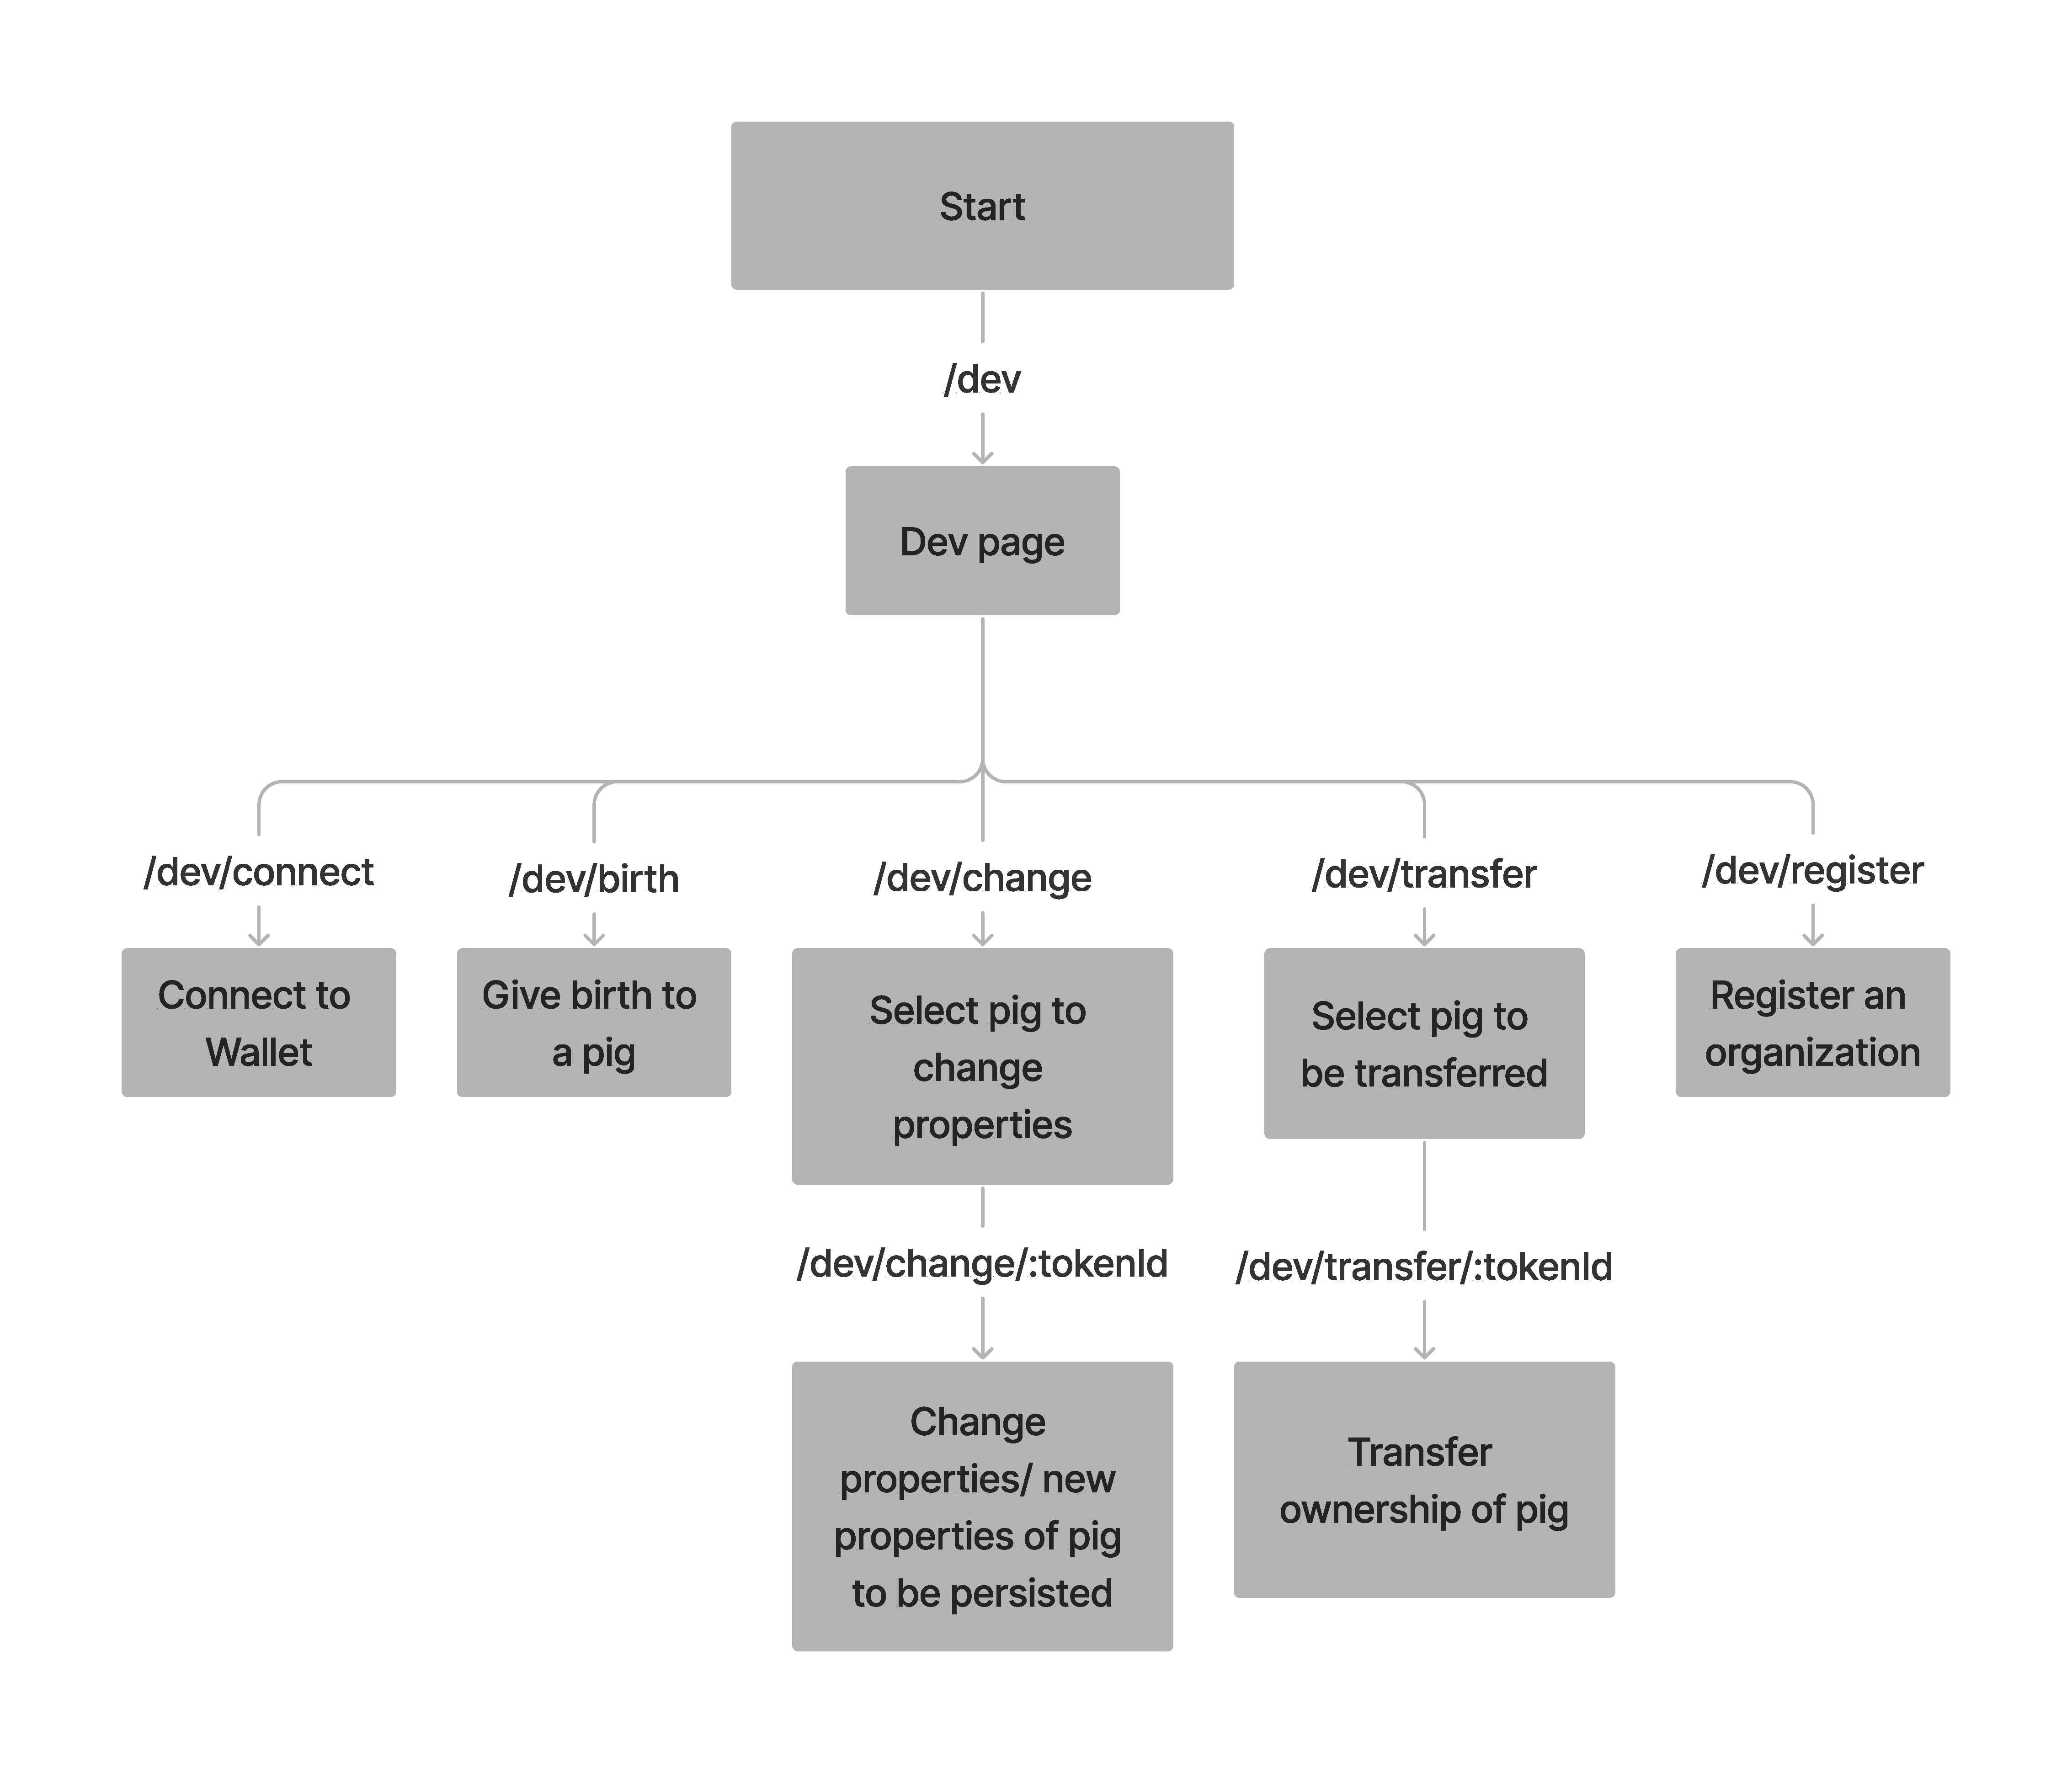
\includegraphics[width=\textwidth]{images/dev_paths.pdf}
    \caption{Dev pages}
    \label{fig:dev_pages}
\end{figure}
\begin{figure}[pt]
    \centering
    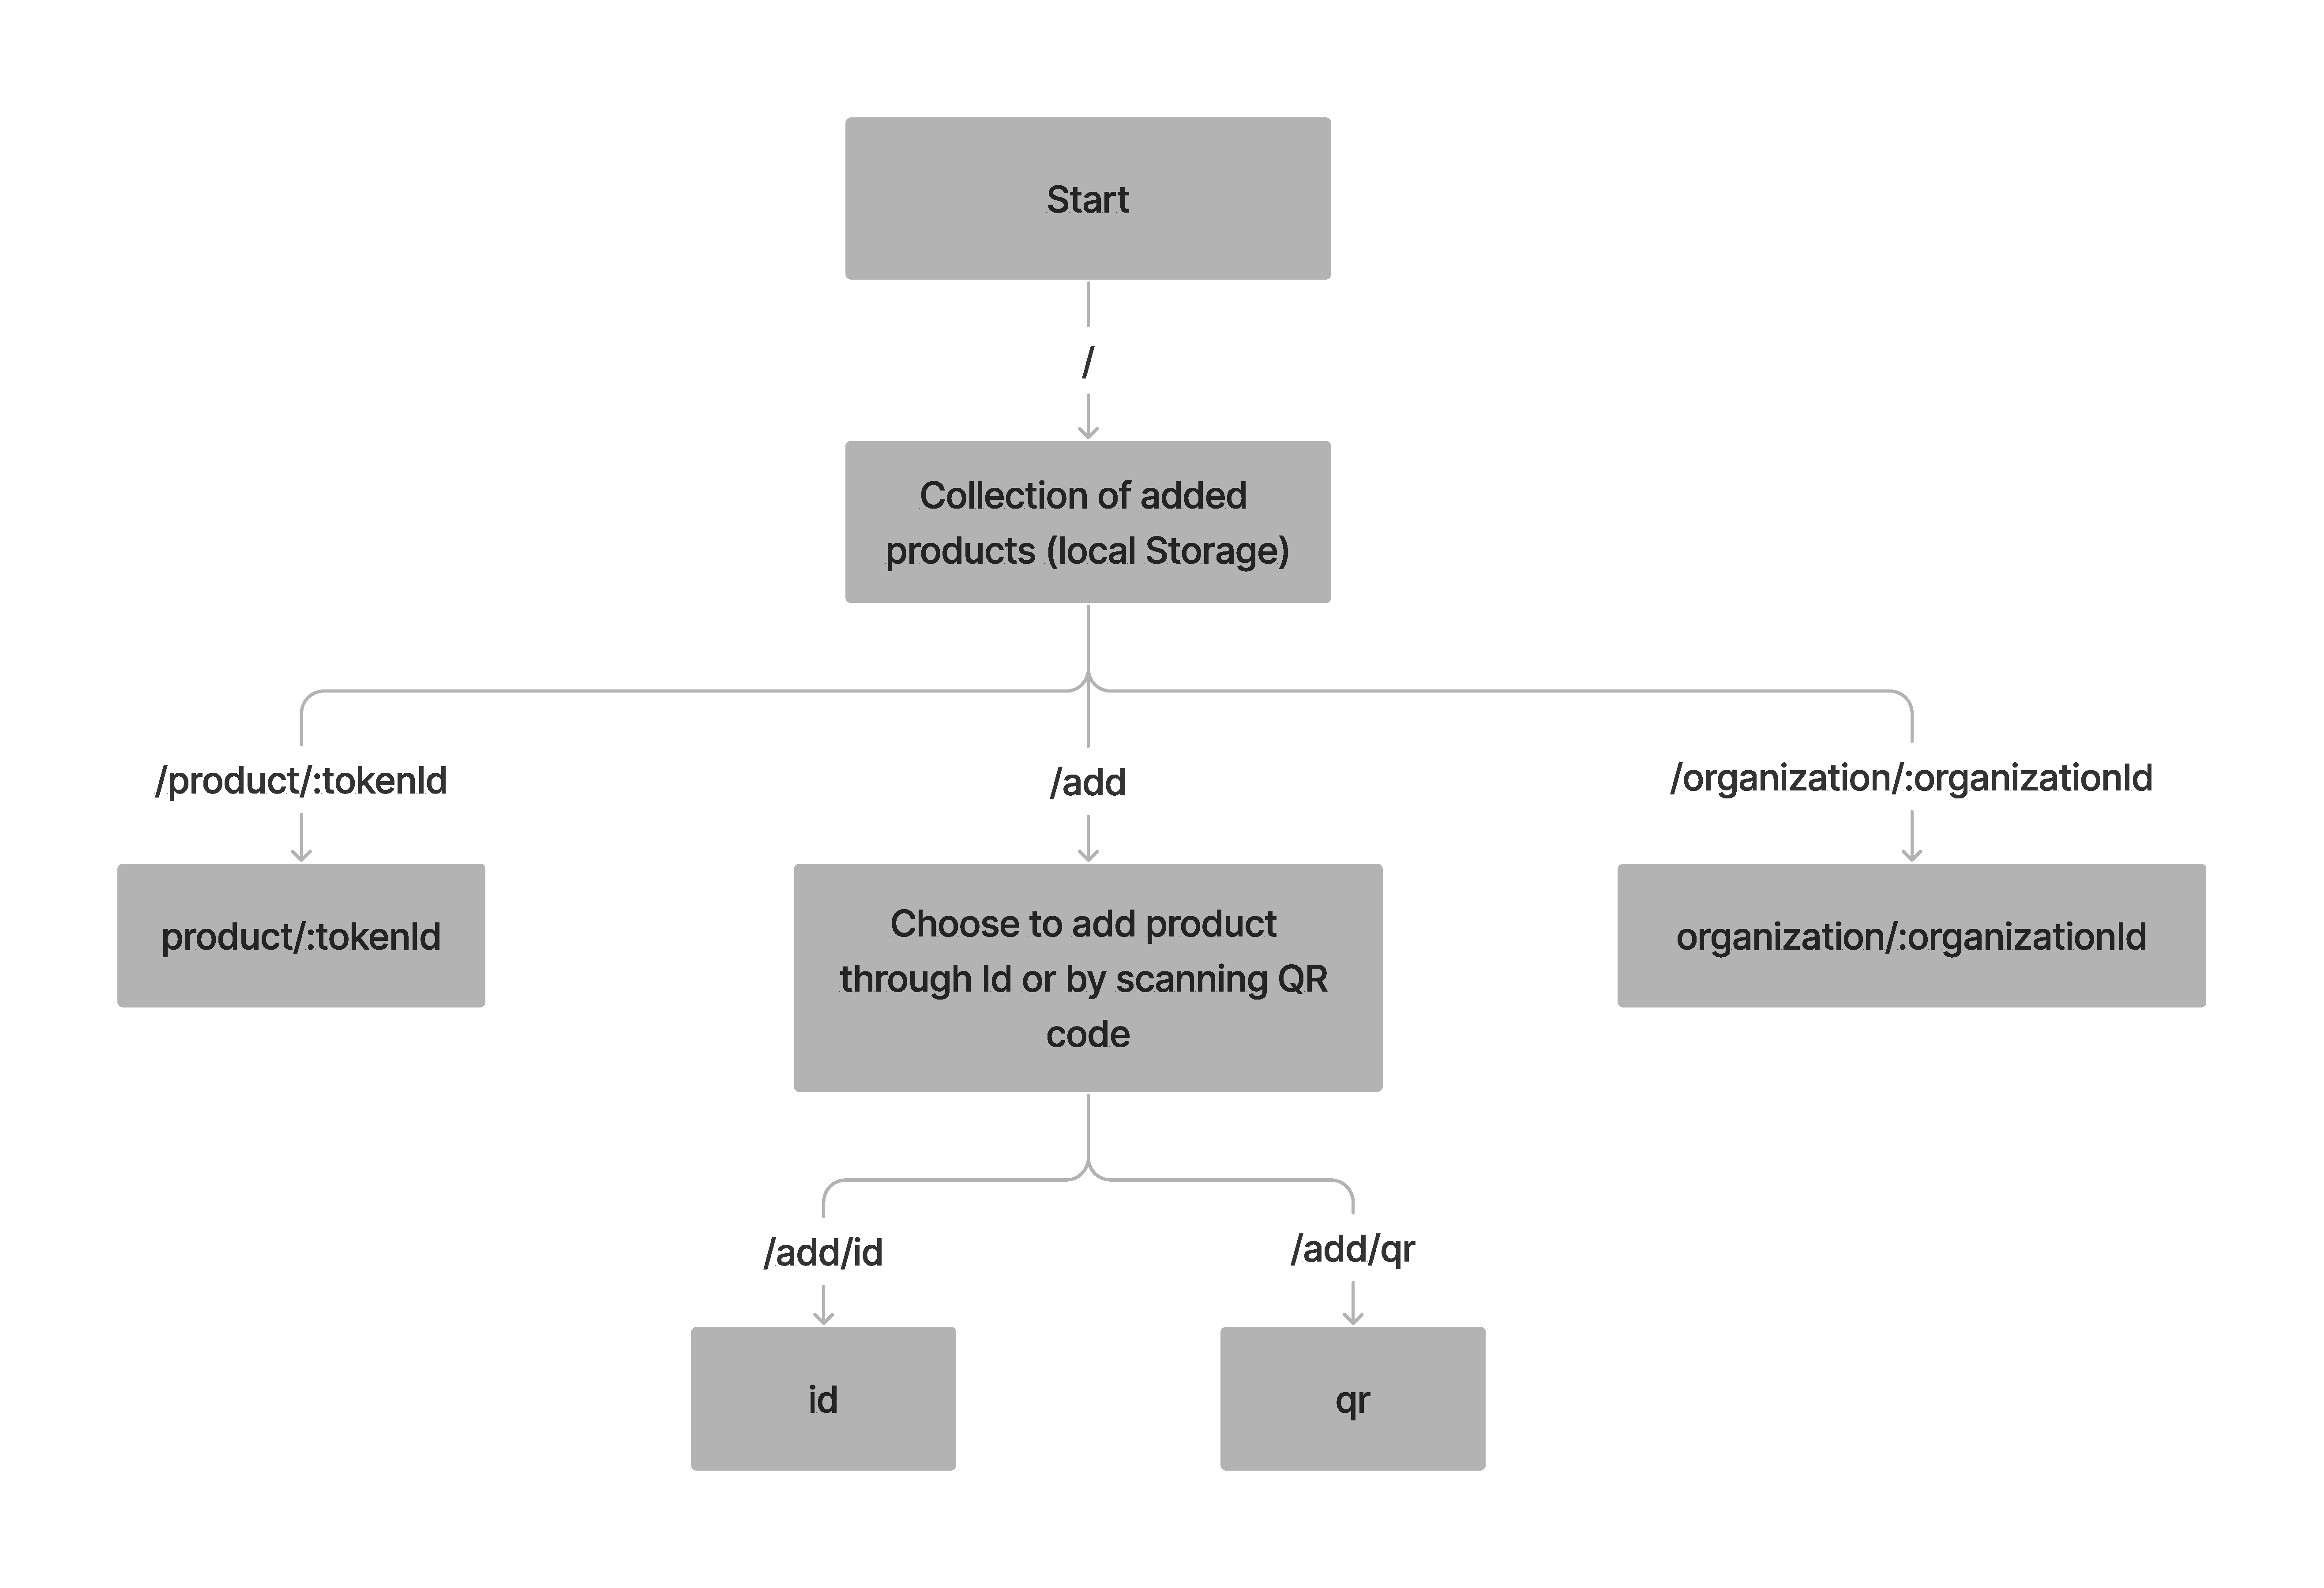
\includegraphics[width=\textwidth]{images/public_paths.pdf}
    \caption{Public pages}
    \label{fig:public_pages}
\end{figure}


\subsection{Dev Pages} \label{se:dev_pages}
The dev pages contain a series of pages that are necessary to quickly interact with the smart contract. In theory, these interaction could also have been modeled and executed through functions in Truffle, however, since any transactions and presentation layer tasks are performed through the web app's \gls{gui}, it is a quick and easy way to perform all of these tasks in the browser. Additionally, this could serve as an entry point for an implementation that would allow producers to implement a \gls{gui} of their own.

The first page listed in the development pages is the "connect" page. It allows producers to connect their wallet and use it for any interactions with the smart contract. Note, that theoretically the consumer would not need a wallet for the public pages as the only actions performed in these pages are "read" actions. However, to keep it simple, the current implementation always requires a connection. This could be adapted through Wagmi's providers.

As soon as a user connected their wallet, they are able to:
\begin{enumerate}
    \item Give birth to a random pig [\textit{/dev/birth}; leverages the \textit{createNewProduct} method]
    \item Select a pig to change properties [\textit{/dev/change}; leverages the \textit{createNewProduct} method]
    \item Select a pig to be transferred to another wallet [\textit{/dev/transfer}; leverages the \textit{transferProduct} method]
    \item Register themselves as an organization (which will allow consumers to see the organization's details) [\textit{/dev/register}; leverages the \textit{requestRegistration} method]
\end{enumerate}

If a developer were to clone a fresh version of the repo and spins up all the containers, a minimum set of actions that would need to be performed to see something relevant would be to first connect their wallet (1.), optionally register themselves as organization (4.\footnote{If not registered, consumers will see an error message when inspecting the organization associated with the product}) and finally give birth to a (random) product/pig. Changing properties and transferring ownership to another entity will show lead to a more realistic supply chain that will also be visualized in the timeline for the consumer. 

\subsection{Public Pages}\label{se:public_pages}
The public pages are consumer facing pages that are meant to be used to keep track of any products acquired in the physical world. As soon as the product is physically available, a consumer has the option to either scan a QR code (not yet implemented, see \ref{se:future_work_frontend}) or to input the product ID (tokenId of the product on the blockchain) to add the product to the watch list. The products that are kept in the watchlist are currently stored in local storage. Persisting the products in such a way can be replaced by any arbitrary solution to persist data such as traditional databases or chrome's sync storage.
Any product saved in the product overview can be viewed in a timeline. The timeline shows all the individual entries of the product in time. From there, a consumer may also see the organizational data that was registered as described in the last section \ref{se:dev_pages}. A few public pages are appended, see figures \ref{fig:timeline_pig}, \ref{fig:list_of_pigs} and \ref{fig:organization}.


\section{Future Work}\label{se:future_work}
In the following section potential enhancements and adaptations for the future iterations of the SPECK system will be explored. We will delve into the options available for the system's expansion, refinement, and further integration. These future possibilities aren't fixed paths but are intended to open up a dialogue about the ongoing evolution of SPECK, aligning it with industry advancements, user expectations, and emerging trends in the food supply chain management. Each option explores the scope of possible improvements, anticipating future demands and preparing SPECK to meet them head on. This iterative approach aims to ensure that SPECK continues to deliver on its promise of transparency, efficiency, and accountability in the meat industry's supply chain. The presented list of solutions is not extensive an only presents a selected amount improvements.

\subsection{View Restriction}
In future versions of the SPECK system, confidentiality requirements would need to satisfy the following non-functional requirements.
While every entity in the SPECK system can access data stored in the distributed ledger, certain exceptions are in place to protect sensitive information.

Specifically, details about the medication of animals during both breeding and mast stages are confidential and solely accessible to companies within the coalition. This is likely due to the sensitive nature of such data and the need to ensure proper use of this information.

Similarly, the weight of animals during the mast stage is also regarded as sensitive information and is only available to coalition companies. Such measures likely reflect the competitive nature of the industry and the importance of maintaining certain data points as confidential.

Post-slaughter data points including findings, pH-value, and fat percentage after slaughter, are also treated with strict confidentiality. These specific data points are vital indicators of the quality and health of the slaughtered animals, and are therefore accessible only to companies within the coalition. This ensures that the information is responsibly managed and used for the appropriate purposes within the industry.


\subsection{Gas Optimization \& Decentralized Data Storage}
One area of future work that can greatly optimize the SPECK system involves the strategic management of data storage in the context of the smart contract. Currently, data is saved directly on the smart contract, which while secure, can result in high gas consumption due to the inherent costs associated with storing and manipulating data on the Ethereum network. A potential solution to this issue is the integration of a decentralized data storage solution such as the InterPlanetary File System (IPFS). IPFS can offer a scalable and efficient method for storing data, allowing the system to maintain its decentralized nature while significantly reducing gas consumption. Instead of storing all data directly on the smart contract, data could be stored on IPFS, and the smart contract would only need to store the IPFS hash pointer to that data. This approach would retain the immutability and transparency of the data, while also improving the overall efficiency and cost-effectiveness of the SPECK system.

\subsection{Change Organization Data}
As part of our continuous improvement efforts, one aspect that requires attention pertains to the flexibility of modifying organization data stored in the OrganizationAuthenticator.sol contract. In the current state of the system, organization data can only be entered once during the registration request process, with no provision for subsequent changes. This rigid model doesn't account for dynamic variables like animal welfare scores or environmental scores, which are subject to fluctuation over time. Therefore, it is crucial to consider a system that allows for the updating of such attributes.

The proposed solution is not about allowing direct alterations to the existing data but introducing an appending system. With this system in place, new data would not overwrite the old, but would instead be added as a new entry, effectively creating a historical record of the organization's data. This would maintain the integrity of the historical data while allowing for real-time updates, thus keeping the system's data reflective of the current status of the organization. Consequently, this system would ensure that the SPECK system remains an accurate and reliable tool for all stakeholders, upholding its mission for transparency and accountability in the meat industry supply chain.

\subsection{Transfer Proposal}
Future improvements to the SPECK system should consider implementing a transfer proposal system within the Speck.sol contract, to ensure transparency and control during the transfer of product ownership. Under the current system, transfers can occur without explicit agreement from both sides, potentially leading to disputes and inconsistencies. A transfer proposal system would allow the current owner to propose a transfer, including all relevant product data and potentially the sale price. The receiving party would then have the opportunity to review and accept this proposal before the transfer is executed.

Incorporating this system into the Speck.sol contract would necessitate a new data structure to store and manage these proposals. This enhancement would not only streamline the process of ownership transfers but also bolster the transparency and accountability of transactions within the system. Ensuring that both parties have a clear understanding and acceptance of the terms of transfer is crucial to maintaining trust and reliability within the SPECK ecosystem.


\subsection{Frontend features}\label{se:future_work_frontend}

Looking towards the future, several key enhancements have been identified to further improve the SPECK system's functionality, usability, and user experience. 
Firstly, integrating an automatic clearing function for the local storage after a set time period would be beneficial. This feature would ensure efficient use of storage resources and maintain optimal system performance.

Secondly, implementing a QR code scanner into the system could significantly streamline data entry and retrieval processes, making it more user-friendly, especially for consumers wanting to quickly access information about a product.

Thirdly, creating a separate repository specifically for producers could provide them with a tailored platform, meeting their unique needs and requirements. This dedicated space would offer producers enhanced usability and an improved, industry-specific experience.

Lastly, a few other important additions have been suggested to further personalize and improve user experience. These include the option for users to use an account to sync data across devices, providing continuity and flexibility. Additionally, introducing settings to customize individual user experiences, such as controlling how long a product is kept in storage, or user interface preferences like dark mode, would give users greater control over their interaction with the SPECK system. 


% Anhang / Appendix
\appendix % Ab hier wird mit A, B, ... weiternummeriert.
% Für den Fall eines Anhangs entkommentieren
\section{Appendix}
\begin{figure}[tbh]
    \centering
    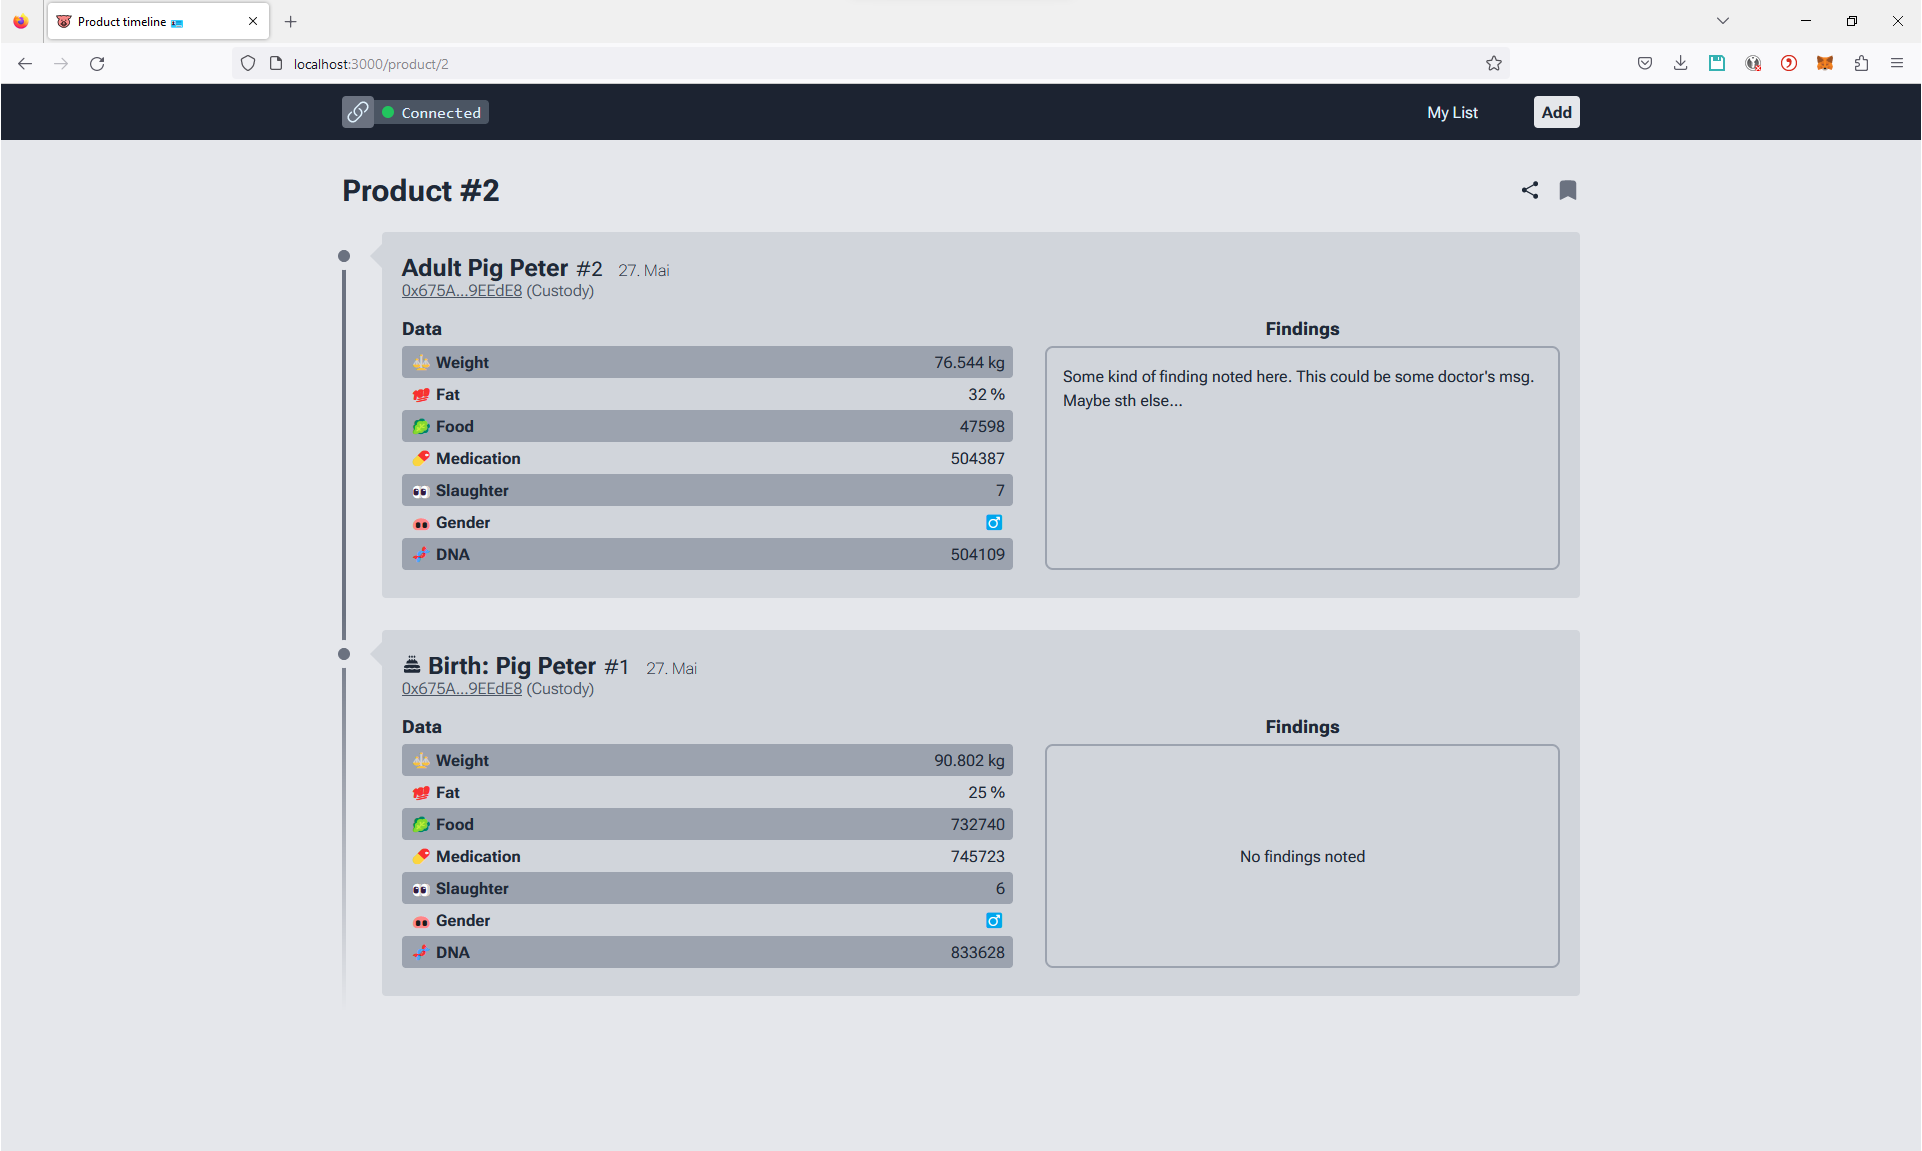
\includegraphics[width=0.82\textwidth]{images/timeline.png}
    \caption{Timeline of a product's chain}
    \label{fig:timeline_pig}
\end{figure}

\begin{figure}[tbh]
    \centering
    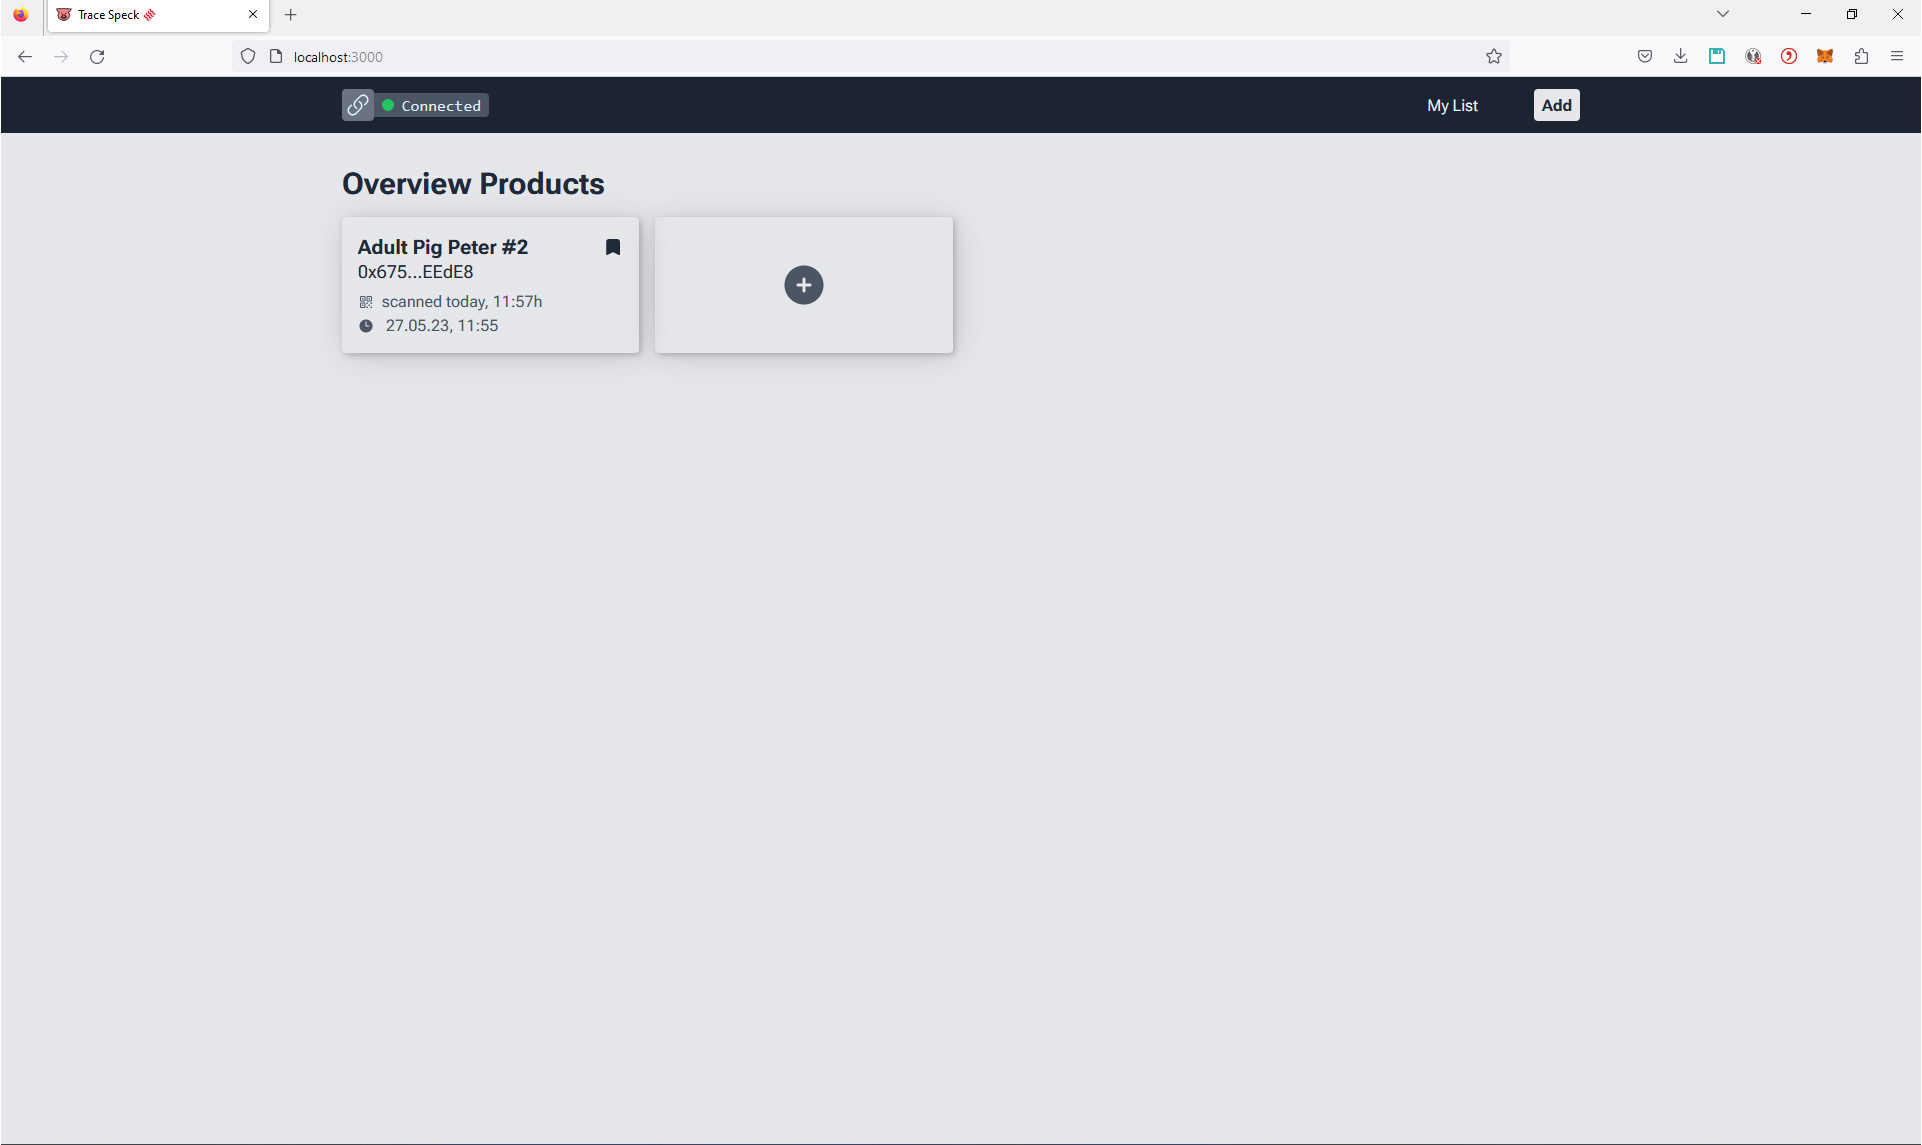
\includegraphics[width=0.82\textwidth]{images/list_pigs.png}
    \caption{Collection of pigs that added to watchlist by consumer}
    \label{fig:list_of_pigs}
\end{figure}


\begin{figure}[tbh]
    \centering
    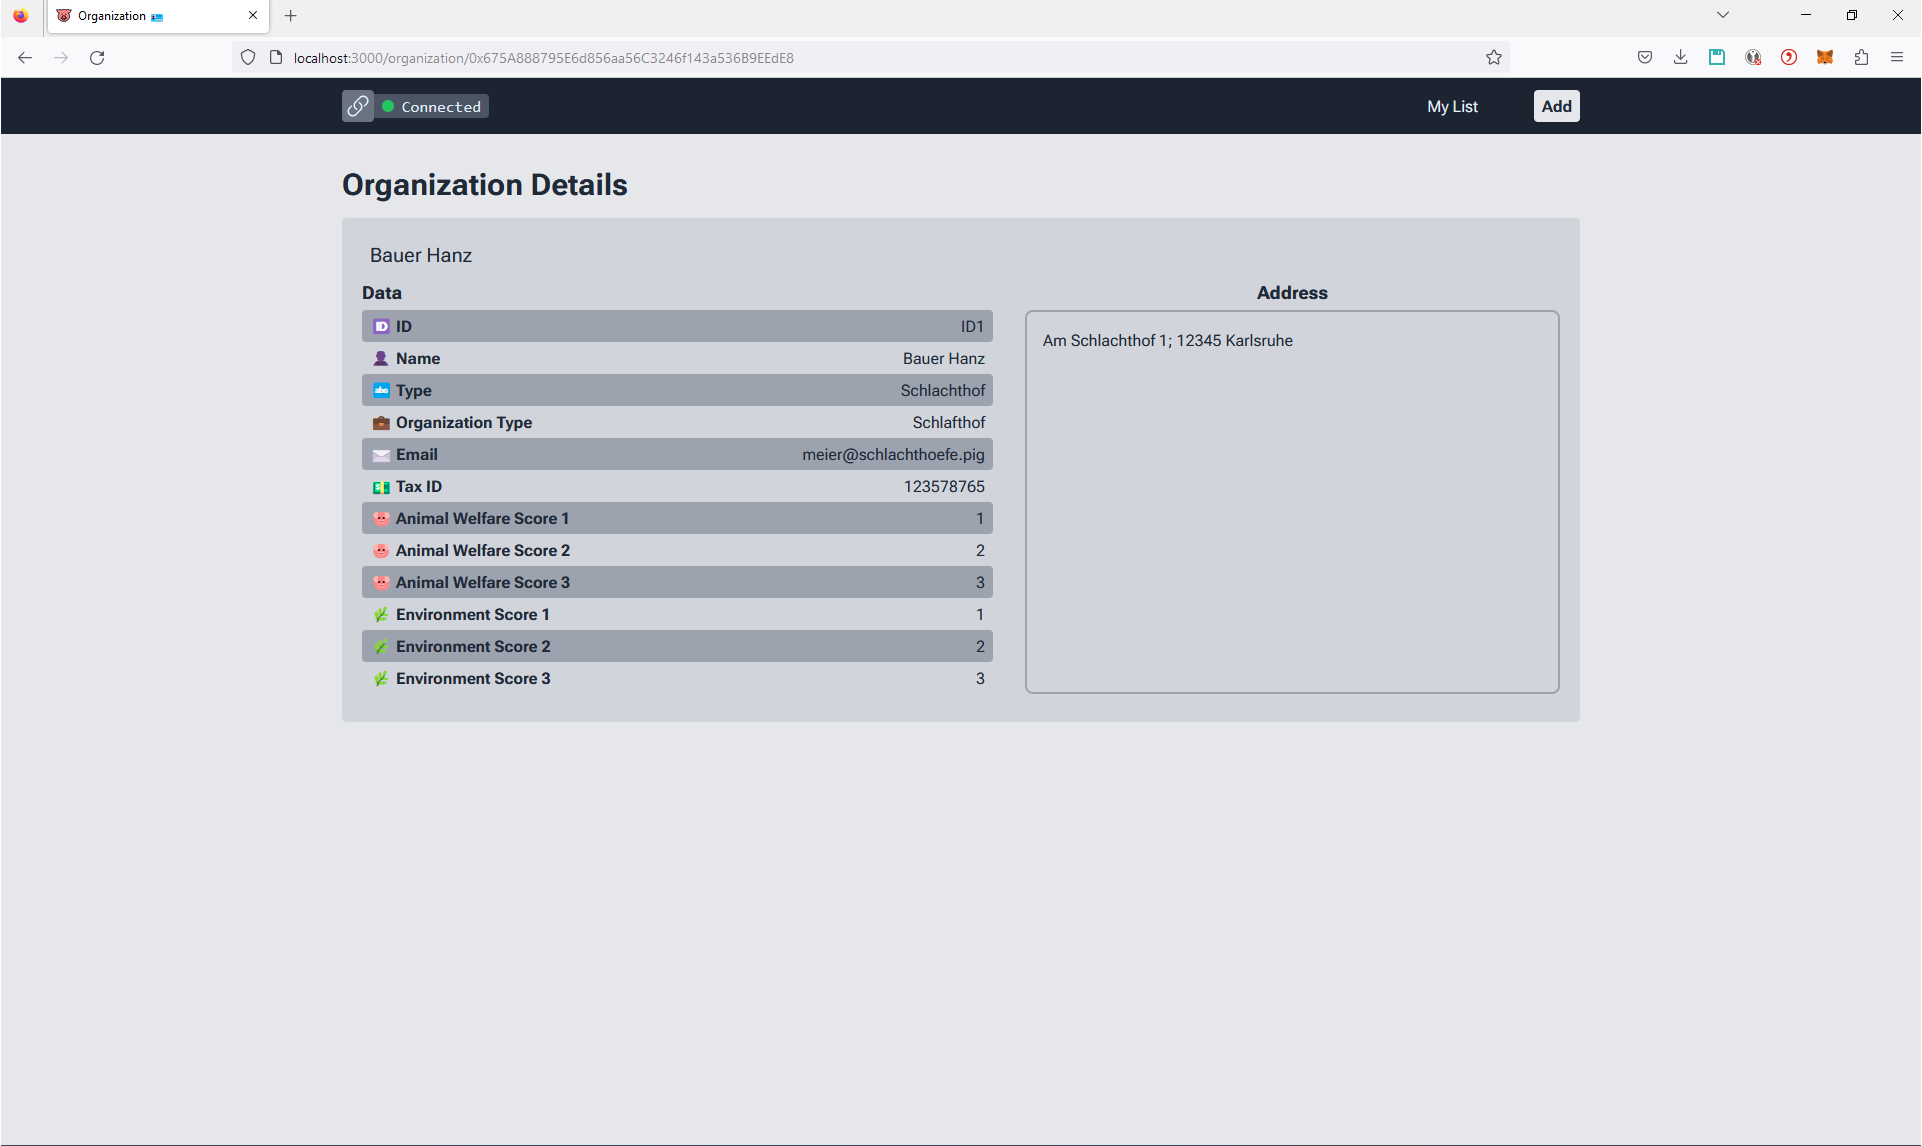
\includegraphics[width=0.82\textwidth]{images/oragnization.png}
    \caption{Registered organization displayed to consumer}
    \label{fig:organization}
\end{figure}

\begin{figure}[bth]
    \centering
    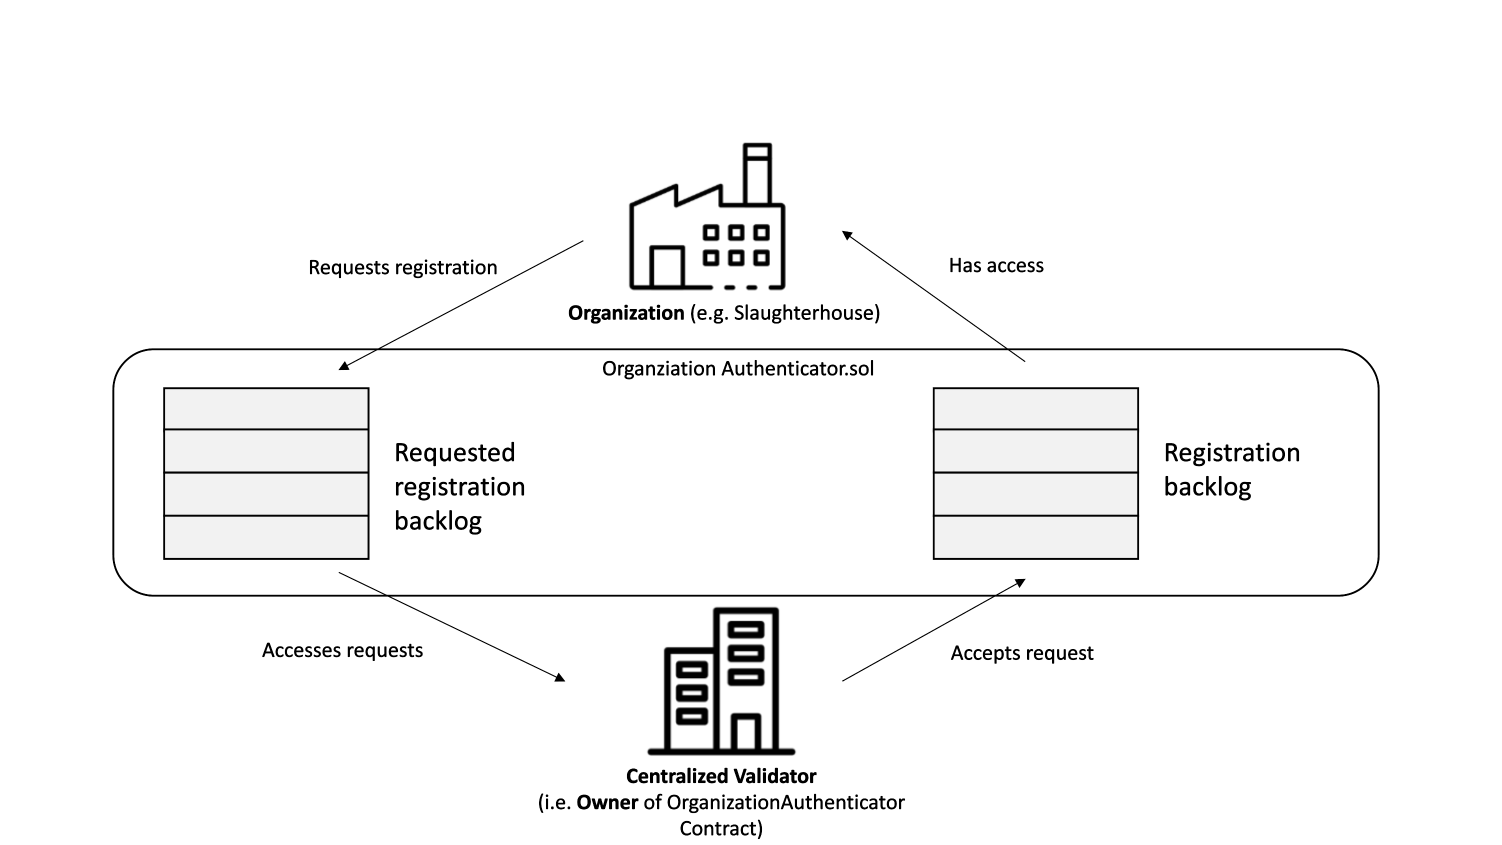
\includegraphics[width=1\textwidth]{images/registration_process.png}
    \caption{Registration process of \textit{OrganizationAuthenticator.sol}}
    \label{fig:registration_process}
\end{figure}

\newpage
\subsection{OrganizationAutheticator.sol}\label{se:organization_authenticator.sol}


\textbf{Imports}

\begin{itemize}
    \item "@openzeppelin/contracts/token/ERC721/ERC721.sol"
    \item "@openzeppelin/contracts/utils/Counters.sol"
    \item  "@openzeppelin/contracts/access/Ownable.sol"
\end{itemize}


\textbf{State Variables}


\begin{table}[H]
\resizebox{\columnwidth}{!}{%
\begin{tabular}{ll}
\textbf{Name}              & \textbf{Description}                                                                   \\
\texttt{\textunderscore orgIds}                    & A counter to track the next open token ID     \\
\texttt{\textunderscore organizationAuthenticator}             & A counter to track the number of registration requests.                                \\
\texttt{\textunderscore registeredAmount}           & A counter to track the number of registered organizations.                             \\
\texttt{\textunderscore registered}                 & A mapping to store the registration status of organizations based on their ID.         \\
\texttt{\textunderscore organizationData}           & A mapping to store organization data based on their ID.                                \\
\texttt{\textunderscore registrationRequested}      & A mapping to track the registration request status of organizations based on their ID. \\
\texttt{\textunderscore addressToId}                & A mapping to associate an organization's Ethereum address with its ID.                 \\
\texttt{\textunderscore registrationRequestedArray} & An array to store the IDs of organizations that have requested registration.          
\end{tabular}%
}
\end{table}

\textbf{Events}


\begin{itemize}
    \item \texttt{\textunderscore Authenticate(string \textunderscore msg)}: Event emitted when an authentication is performed.
    \item \texttt{\textunderscore RegistrationRequested(address indexed requestAddress)}: Event emitted when a registration request is made.
\end{itemize}



\textbf{Structs}

\texttt{Organization}: A struct to hold organization data
\begin{table}[H]
\begin{tabular}{ll}
\textbf{Attribute}     & \textbf{Datatype} \\
\texttt{id}                     & string            \\
\texttt{name}                   & string            \\
\texttt{type\textunderscore}                  & string            \\
\texttt{organization\textunderscore type}      & string            \\
\texttt{email}                  & string            \\
\texttt{institution\textunderscore type}       & string            \\
\texttt{address\textunderscore}              & string            \\
\texttt{tax\textunderscore id}                 & uint256           \\
\texttt{animal\textunderscore welfare\textunderscore score\textunderscore 1} & uint256           \\
\texttt{animal\textunderscore welfare\textunderscore score\textunderscore 2} & uint256           \\
\texttt{animal\textunderscore welfare\textunderscore score\textunderscore 3} & uint256           \\
\texttt{environment\textunderscore score\textunderscore 1}    & uint256           \\
\texttt{environment\textunderscore score\textunderscore 2}    & uint256           \\
\texttt{environment\textunderscore score\textunderscore 3}    & uint256           \\
\texttt{creation\textunderscore right}        & bool             
\end{tabular}
\end{table}




\textbf{Modifiers}
\begin{itemize}
      \item \texttt{\textunderscore onlyOwner} \textit{(from ERC721)}: Modifier that restricts access to the contract owner.
\end{itemize}

\textbf{Methods}
\begin{table}[H]
\resizebox{\columnwidth}{!}{%
\begin{tabular}{lll}
\textbf{Name} &                   & \textbf{Description}                                                                                           \\ \hline
\texttt{authenticateById} & \textbf{@dev}     & Check if the organization with the given ID is registered.                                       \\
                          & \textbf{@params}  & \texttt{\_orgId}: ID of the organization to check authentication status.                                         \\
                          & \textbf{@returns} & A boolean indicating if the organization is registered or not.                                       \\
                          &                   &                                                                                                                \\ \hline
\texttt{authenticate} & \textbf{@dev}     & Check if the organization with the given address is registered.                                                    \\
                          & \textbf{@params}  & \texttt{\_address}: Address of the organization to check authentication status. \\
                          & \textbf{@returns} & A boolean indicating if the organization is registered or not.                                                 \\
                          &                   &                                                                                                                \\ \hline
\texttt{requestRegistration} & \textbf{@dev}              & Request registration for a new organization.                                                                   \\
                          & \textbf{@params}           & \texttt{\_data}: Struct containing organization data to register                                                           \\
                          &                   &                                                                                                                \\ \hline
\texttt{register} & \textbf{@dev}              & Register an organization.                                                                                      \\
                          & \textbf{@params}           & \texttt{\_orgId}: ID of the organization to register                                                                     \\
                          &                   &                                                                                                                \\ \hline
\texttt{getRequestedRegistrations} & \textbf{@dev}              & Get a list of organization requests.                                                                           \\
                          & \textbf{@returns}           & An array of organizations                                                                                          \\
                          &                   &                                                                                                                \\ \hline
\texttt{getMyData} &      \textbf{@dev}        & Get the organization data from \textit{msg.sender}                                                           \\
                          & \textbf{@returns}           & Organization data of the \texttt{msg.sender}                                                                     \\
                          &                   &                                                                                                                \\ \hline
\texttt{amIRegistered} &        \textbf{@dev}      & Check if the \textit{msg.sender} is registered                                                             \\
                          & \textbf{@returns}           & A boolean indicating if the \texttt{msg.sender} is registered or not                                                                      \\
                          &                   &                                                                                                                \\ \hline
\texttt{getOrganizationDataByAddress} &      \textbf{@dev}        & Get the organization data of a given address                                                                 \\
                          & \textbf{@params}           & \texttt{\_address}: Address of the organization to retrieve data for                                                           \\
                          & \textbf{@returns}           & Organization data of the given address                                                                 \\
                          &                   &                                                                                                                \\ \hline
\texttt{totalRequestedOrganizationAmount} &      \textbf{@dev}        & Get the total number of organization registration requests                                                                           \\
                          & \textbf{@returns}           & The total number of organization registration requests                                                                      \\
                          &                   &                                                                                                                \\ \hline
\texttt{totalRegisteredOrganizationAmount} &      \textbf{@dev}        & Get the total number of registered organizations                                                                 \\
                          & \textbf{@returns}           & The total number of registered organizations                                                                      \\
                          &                   &                                                                                                                \\ \hline
\end{tabular}%
}
\end{table}

\newpage
\subsection{Speck.sol}\label{se:speck.sol}
\textbf{Imports}

\begin{itemize}
    \item "@openzeppelin/contracts/token/ERC721/ERC721.sol"
    \item "@openzeppelin/contracts/utils/Counters.sol"
    \item  "@openzeppelin/contracts/access/Ownable.sol"
\end{itemize}


\textbf{State Variables}


\begin{table}[H]
\resizebox{\columnwidth}{!}{%
\begin{tabular}{ll}
\textbf{Name}              & \textbf{Description}                                                                   \\
\texttt{\textunderscore tokenIds}                    & A counter to track the next open token ID.      \\
\texttt{\textunderscore organizationAuthenticator}             & Instance of the OrganizationAuthenticator contract.                                \\
\texttt{\textunderscore products}           & A mapping for storing product data.                           \\
\texttt{\textunderscore tokenOwner}                 & A mapping for storing the owner of a product.        \\       
\end{tabular}%
}
\end{table}

\textbf{Events}
\begin{itemize}
    \item \texttt{\textunderscore NewProductCreated(uint256 indexed tokenId, address indexed owner)}: Event emitted when a new product is created
\end{itemize}



\textbf{Structs}

\texttt{Product}: Struct for storing product information
\begin{table}[H]
\begin{tabular}{ll}
\textbf{Attribute}     & \textbf{Datatype} \\
\texttt{id}                     & string            \\
\texttt{rfid}                   & string            \\
\texttt{genetics}                  & string            \\
\texttt{gender}      & uint256            \\
\texttt{slaughter\textunderscore method}                  & uint256            \\
\texttt{findings}       & string            \\
\texttt{ph\textunderscore value}              & uint256            \\
\texttt{product\textunderscore type} & string           \\
\texttt{animal\textunderscore weight\textunderscore g} & uint256           \\
\texttt{fat\textunderscore percentage} & uint256           \\
\texttt{feed} & string           \\
\texttt{medication}    & string           \\
\texttt{timestamp}    & string           \\     
\end{tabular}
\end{table}



\textbf{Modifiers}
\begin{itemize}
      \item \texttt{\textunderscore onlyRegistered}: Modifier that restricts function calls to authenticated organizations.
      \item \texttt{\textunderscore previousProductCheck}: Modifier that checks if the previous product in the chain exists and belongs to the caller.
\end{itemize}

\textbf{Methods}

\begin{table}[H]
\resizebox{\columnwidth}{!}{%
\begin{tabular}{lll}
\textbf{Name} & \textbf{@dev} & \textbf{Description} \\ \hline
\texttt{createNewProduct} & \textbf{@params} & \texttt{\_product\_data}: The Product struct containing the details of the new product to be created. \\ \hline
\texttt{transferProduct} & \textbf{@params} & \texttt{\_product\_data}: The Product struct containing the details of the product to be transferred. \\
 & \textbf{@params} & \textit{\_to}: The address of the new owner of the product. \\ \hline
\texttt{getProductData} & \textbf{@params} & \texttt{\_tokenId}: The ID of the product to retrieve data for. \\
 & \textbf{@returns} & A tuple containing the Product struct of the product, its token ID, and its current owner. \\ \hline
\texttt{getMultipleProductData} & \textbf{@params} & \texttt{\_token\_ids}: An array of product IDs to retrieve data for. \\
 & \textbf{@returns} & A tuple containing arrays of Product structs, token IDs, and current owners for the specified products. \\ \hline
\texttt{getProductHistory} & \textbf{@params} & \texttt{\_tokenId}: The ID of the product to retrieve the history for. \\
 & \textbf{@returns} & A tuple containing arrays of Product structs, token IDs, and current owners for each version of the product in reverse chronological order. \\ \hline
\texttt{getHistoryDepth} & \textbf{@params} & \texttt{\_tokenId}: The ID of the product to calculate the history depth for. \\
 & \textbf{@params} & \texttt{\_counter}: A counter variable used to keep track of the depth. \\
 & \textbf{@returns} & The depth of the product history. \\ \hline
\texttt{totalProductAmount} & \textbf{@returns} & The total number of products. \\ \hline
\texttt{getOwnerOf} & \textbf{@params} & \texttt{\_tokenId}: The ID of the product to retrieve the owner for. \\
 & \textbf{@returns} & The address of the current owner of the product. \\ \hline
\end{tabular}%
}
\end{table}


% \clearpage
% \input{transcripts/teilnehmer_1_reworked.tex}
% \clearpage
% \input{transcripts/teilnehmer_2}
% \clearpage
% \input{transcripts/teilnehmer_3}
% \clearpage
% \subsection{Interview scenarios}
% \includepdf[
%     pages=-,
%     frame,
%     nup=1x2,
%     delta=10pt 10pt,
%     scale=.9,
%     pagecommand={}
%  ]{interview_scenarios/Battle Cards.pdf}

% Literaturverzeichnis
\bibliographystyle{apalike}
\newpage
\bibliography{YOUR_thesis} % Datei mit Literaturangaben einbinden

% Schriftliche Erklärung
\newpage
% \mbox{}\thispagestyle{empty}

\vspace*{1cm}

{\Large \textbf{\ifthenelse{\boolean{english}}{Assertion}{Erklärung}}} 

\bigskip

\ifthenelse{\boolean{english}}
{\selectlanguage{english}
\textit{Ich versichere wahrheitsgemäß, die Arbeit selbstständig verfasst, alle benutzten Hilfsmittel vollständig und genau angegeben und alles kenntlich gemacht zu haben, was aus Arbeiten anderer unverändert oder mit Abänderungen entnommen wurde sowie die Satzung des KIT zur Sicherung guter wissenschaftlicher Praxis in der jeweils gültigen Fassung beachtet zu haben.}}
{\selectlanguage{ngerman}
\textit{Ich versichere wahrheitsgemäß, die Arbeit selbstständig verfasst, alle benutzten Hilfsmittel vollständig und genau angegeben und alles kenntlich gemacht zu haben, was aus Arbeiten anderer unverändert oder mit Abänderungen entnommen wurde sowie die Satzung des KIT zur Sicherung guter wissenschaftlicher Praxis in der jeweils gültigen Fassung beachtet zu haben.}}

\vspace{1cm}

%
%WICHTIG: Prüfen Sie unbedingt, ob der Text der Erklärung mit der jeweils für den Studiengang aktuell gültigen SPO übereinstimmt!
%
%TODO: Datum der Erklärung angeben
%            Hinweis: Das Datum der Erklärung ist üblicherweise das Abgabedatum
%
%TODO: Eigenen Vornamen und Nachnamen angeben
%
Karlsruhe, \today \hfill VORNAME NACHNAME

%\thispagestyle{empty}\cleardoublepage

%\mbox{}\thispagestyle{empty}
 todo include assertion in real paper

\end{document}